% Options for packages loaded elsewhere
\PassOptionsToPackage{unicode}{hyperref}
\PassOptionsToPackage{hyphens}{url}
%
\documentclass[titlepage, 8pt, a5paper]{ltjsarticle}
\title{虚無・無知・飢餓\\―不安の時代における諸学の綜合―}
\author{Aoko Yano}
\date{2024-09-22}
\usepackage{amsmath,amssymb}
\usepackage{iftex}
\ifPDFTeX
  \usepackage[T1]{fontenc}
  \usepackage[utf8]{inputenc}
  \usepackage{textcomp} % provide euro and other symbols
\else % if luatex or xetex
  \usepackage{unicode-math} % this also loads fontspec
  \defaultfontfeatures{Scale=MatchLowercase}
  \defaultfontfeatures[\rmfamily]{Ligatures=TeX,Scale=1}
\fi
\usepackage{lmodern}
\ifPDFTeX\else
  % xetex/luatex font selection
\fi
% Use upquote if available, for straight quotes in verbatim environments
\IfFileExists{upquote.sty}{\usepackage{upquote}}{}
\IfFileExists{microtype.sty}{% use microtype if available
  \usepackage[]{microtype}
  \UseMicrotypeSet[protrusion]{basicmath} % disable protrusion for tt fonts
}{}
\makeatletter
\@ifundefined{KOMAClassName}{% if non-KOMA class
  \IfFileExists{parskip.sty}{%
    \usepackage{parskip}
  }{% else
    \setlength{\parindent}{0pt}
    \setlength{\parskip}{6pt plus 2pt minus 1pt}}
}{% if KOMA class
  \KOMAoptions{parskip=half}}
\makeatother
\usepackage{xcolor}
\setlength{\emergencystretch}{3em} % prevent overfull lines
\providecommand{\tightlist}{%
  \setlength{\itemsep}{0pt}\setlength{\parskip}{0pt}}
\setcounter{secnumdepth}{-\maxdimen} % remove section numbering
\usepackage{bookmark}
\IfFileExists{xurl.sty}{\usepackage{xurl}}{} % add URL line breaks if available
\urlstyle{same}
\hypersetup{
  hidelinks,
  pdfcreator={LaTeX via pandoc}}
\begin{document}
\maketitle


本稿において、「序論」が「問題設定とそれに対する答え方の構え」を示すものである一方で、「緒言」は「本稿が書かれた時代の知の配置の中で、本稿がどのような位置づけの考察なのか」を示すものだ。本稿は、誰に何をもたらすのか。そして、それを可能にするために何をするのか。

本稿がまず念頭においている読者は、私たちを駆り立てるべくますます騒がしさを増してきつつある世の喧騒に対してうんざりしつつも、実際のところどのように生きるべきかについて思いめぐらせている人々だ。そうした人々にとって、本稿は静寂を取り戻す助けとなることだろう。本稿は、人々が混乱の中に沈むことを防ぐ小舟のような存在となるに違いない。その小舟の上からは、世の喧騒が如何に簡単な無理解に立脚したものであるかがすぐに分かるようになる。そして読者は、本稿を読むことで、本質的に未解決な問題については地道な探究を重ねるしかなく、そこに魔法のような解決があることは稀なのだと、腹の底から納得できるようになるだろう。

このようにして得られる静寂において、読者の前にはこの宇宙の中で、私たちが如何に小さな存在であるかが分かるようになる。そこでは宇宙が、古の人間が思い描いたであろうような意味に満ちたものではなく、茫漠とした無根拠と無意味として現れてくる。

しかし、それにもかかわらず、読者はそこでただ単にすべてから切り離された根無し草になるわけではない。読者はそこで、自身の身体に出会う。その身体とは、自身がそこでそのように感じ、そう欲する以外の仕方では欲することができないような「固着した飢え」である。

飢えは救いではないが、飢えを無視することは苦しみを生む。固着した飢えという立脚点を得て、その渇きを癒すために、幸運ならば、読者は本稿という知識の小舟から無知が渦巻く宇宙という大海へと最後は飛び込むだろう。本稿が提供する知識の体系は、その際に自身の身を混沌から守る一助にもなるだろう。本稿は、そのようなものだ。

そのような議論を、本稿はどのようにして可能にするのか。それは、本稿は複数の専門分野で発見された知識を相互に束縛させあい、接続させあうことによってだ。そうすることで、本稿は複数の専門分野を一つに繋ぎ合わせ、統合的な知の道筋を浮かび上がらせる。その際に、本稿は各専門分野の基本的な知識しか用いない。それは、本稿が示す道筋が、実は現代人の眼前に当然のごとく在り続けていたにもかかわらず、ほとんど誰にも顧みられなかったものだからだ。この意味で、本稿は特定の専門分野に直接寄与するものではないし、文学的なテクストによって人々の情動を揺さぶるものでもない。それらは本稿の目的ではないからだ。同様に、特定の専門分野への寄与や文学的なテクストを期待する読者に、本稿が与えられるものはない。それにもかかわらず、本稿が示す道筋は、現代人の知識を整理することによって、様々な専門分野や文学に従事する人々を含む幅広い層に寄与するだろう。

\newpage

\section{序論:本稿の意義}\label{ux5e8fux8ad6ux672cux7a3fux306eux610fux7fa9}

\subsection{問題意識あるいは問いの設定}\label{ux554fux984cux610fux8b58ux3042ux308bux3044ux306fux554fux3044ux306eux8a2dux5b9a}

世界のすべてについて知ることができる立場が、広く人々に与えられたことはない。それゆえに、人々はこれまで常に無知を抱え、その無知ゆえに世界に翻弄され、困惑し、そして不安を抱えてきた。不条理な現実、耐えがたい受苦、取り返しのつかない過去の過ちへの後悔\ldots\ldots これらを浴びせられたときに、それが「無駄(umsonst)」であるなどとは、到底受け入れがたいものだ{[}\^{}1{]}。人が不可解な自身の生について、「何も欲さない」でいることは至難の業である{[}\^{}2{]}。人は、飢えているのだ。

そこで、人々は「無を欲する」ことにした{[}\^{}3{]}。自身の知を超えた彼方に崇高なるものの存在を措定し、そこから惨めな己の生に救いの光を当てることにしたのだ。自然界の、血族の、国家の、人類の神性が信じられ、また超越的な神が信じられるようになった。それらが真に実在するかどうかなどは、人間には知るべくもない。しかし、信じるだけでも、そこに「意味」が与えられ、それによって人の心は救われるのだ。

だが、かつて信じられた物語の多くは、科学的営為の積み重ねによる人類の知の増加によって、寓話として捉えるのでもなければ、あまりにも迷信的なものに見えるようになってしまった。それでも、まだかつて人類が希望を失わない時代があった。

それは、「希望に満ちた未来」という物語が代わりに信じられるようになったからだ。新しく人々の前面に現れた資本主義という「欲求の体系{[}\^{}4{]}」においては、貨幣などの通用力を持つ媒介を用いることで、人々の不満と生産力とがボトムアップで調整されながら、ますます人類の力が増していった。そこで必要なのは、暴力的な破壊や盗みを合理的な行動選択として成立させないための安全保障体制だけ、のはずだった。しかし、この動的な物語もまた、瓦解を始めることになった(=「大きな物語の終焉」{[}\^{}5{]})。

まず第一に、20世紀後半になると、無尽蔵にも思われた地球の資源および環境が、人類の活動によって大いに攪乱されうるものであり、ナイーブにそれらを収奪し続けていては文明は維持できなくなるかもしれないのだということが分かってきた。人類の果てしない進歩を漫然と信じられる時代は終わってしまった。「存続するための十分な努力ができなければ、廃れ、やがては滅びるかもしれない」という未来が見えてきたのである。

続いて第二に、21世紀に入ると、科学技術は高度な教育なしではとても信じられないような水準に達するようになった。世界と社会のフロンティアは魔術的{[}\^{}6{]}になり、そうしたフロンティアを理解するだけのリテラシーがない者は、わけもわからず時代の流れに振り回されるようになっていった。それは新たな「疎外」状況であり、その疎外の中で「社会から見捨てられた」と反感を溜め込む者たちも多く現れるようになった。

そして第三に、2010年代以降、玉石混交の情報がインターネットを通じて社会に氾濫するようになった。前世紀に比すれば世界は概ね豊かになった{[}\^{}7{]}ものの、世界各地の酸鼻極まる悲惨が事実として存在しており、人々はそうしさ悲惨についての情報を毎日のように浴びせられている。悲惨がなくならない以上、再びそこに「なぜ?」という問いが持ち上がる。そして、その問いに対しては「その悲惨の背後に邪悪な陰謀を張り巡らせる権力者がおり、説得など通じないならず者がおり、私服を肥やすことにしか関心のない悪徳商人がおり\ldots\ldots」といった物語が与えられることになるわけだ。もちろん、そうした物語りは気に食わない他者の信用を毀損するための偽情報にすぎない場合が少なくない(なお、本当にそうした陰謀や悪が実在する場合もある)のだが、そうした物語を魅力的に感じる人は後を絶たず、今日ではそうした偽情報の氾濫にまつわる混乱が社会問題となっている。しかも、そこでは混乱した状況に対して「もう何も分からん、とりあえず社会が変化するのは何やら恐ろしいからやめてくれ!」と判断させることを目標にしたメタな連中すらもいる始末だ(=「ディスインフレーション」{[}\^{}8{]})。

要するに、過去より存在する物語を信仰し続けるのには筋金入りの信心が必要であり、ナイーブに未来を信じるのには事態は差し迫りすぎており、真面目に社会を前進させるには人類の平均的知力は既に「落伍しないのがやっと」のレベルになっていて、かつ現に取りこぼされた人々が「救い」として縋りつくのは(世界に溢れる悲惨を直に引き受けるのでなければ)往々にして陰謀論的な「真実」であったりする\ldots\ldots という有様なのだ。

結局、人類は自身の不安と悲しみを慰撫するための新たな物語を渇望し続けている。人間の歴史とは、無を仰ぐ「ニヒリズム」の歴史であった。本論にて詳述するが、人類がさらに進化したとしても、おそらくこれからも―少なくとも当分は―そうだろう。

\begin{itemize}
\tightlist
\item
  {[}\^{}1{]}
  um-sonst(無を-狙う)ものとしての無駄については、ニーチェのいわゆる「レンツァーハイデ草稿」(ニーチェ(1974=1984:275-284)所収の「1886年夏―1887年秋 5[71]」に相当)を参照。
\item
  {[}\^{}2{]} ニーチェ(1887=1940:271)を参照。
\item
  {[}\^{}3{]} 同上
\item
  {[}\^{}4{]} ==ヘーゲル『法の哲学』==を参照。
\item
  {[}\^{}5{]}
  言葉としての「大きな物語の終焉」はリオタール(1979=1989)で提唱された。その本稿における意味合いとしては松本(2018:15-16)を参照。
\item
  {[}\^{}6{]} 落合(2015)を参照。
\item
  {[}\^{}7{]} ロスリング/ロスリング/ロンランド(2018=2019)を参照。
\item
  {[}\^{}8{]}
  陰謀論とディスインフレーションについては、小泉/桒原/小宮山(2023)における記述と、津田(2024)における「これは権威主義国家でよく使われる手法なんですけど、ウソか本当か分らない情報を、ソーシャルメディアなどを使ってとにかく大量に流すんですね。すると人びとはどの情報を信じればよいかわからず、変化よりも現状維持を選ぶようになると。つまり、権力者が自分たちの体制を維持しようと思ったら、まじめに説得するより、訳のわからない情報を流して思考停止にさせた方が、人びとを楽にコントロールできるというわけです」という記述を参照。
\end{itemize}

\subsection{本稿の目的あるいは目論見}\label{ux672cux7a3fux306eux76eeux7684ux3042ux308bux3044ux306fux76eeux8ad6ux898b}

本稿には、三つの目標がある。本稿はその三つの目標を達成することによって、先述したような状況の中で人々がより広く「満足」できる社会を構想することを目的としている。

第一の目標は、人類において不満と満足が現れるダイナミズムをモデル化して示すことだ。人はどのようなときに不満を覚え、どのようにして満足を得るのか。その仕組みのどこが必然的なものであり、どこがそうではないのか。それを科学的な知見に基づいて明らかにするのがこの第一の目標だ。そこでは、物語を信じることには不満を解消し満足を獲得する上での様々な有効性があり、それゆえに「信じるに値する物語を獲得すること」が効果的なのだということも説かれる。この目標が達成されることで、以下の第二の目標を目指すことができるようになる。
第二の目標は、同じく科学的な知見に基づいて「新しい物語が満たすべき基準としての『推奨ボーダーライン』」を引くことにある。それは、それを満たすことで科学的な知見とその物語とが整合的であることを意味するようなボーダーラインである。ここで、「推奨ボーダーライン」という歯切れの悪い表現をしているのには理由がある。「推奨」という語と「ボーダーライン」という語のそれぞれについて、その語を採用した二つの理由を以下で説明する。

まず第一に、「ボーダーライン」という語を選んだ意味についてだが、これは(少なくとも現時点における人類の)科学的知見は世界の全貌を解き明かすような水準には達していないため、その総体を集成してもそれで世界の全貌について説明してくれる物語が即座に生み出されるわけではないという事情から説明される。すなわち、科学的知見と整合的な物語を志向するにしても、本稿が提示しようとするボーダーラインはあくまでそうした物語の「必要条件」に留まることになるのだ。この必要条件を満たす物語を立ち上げるにしても、本稿が示すボーダーラインの範囲を超えた「肉付け」や「選択」の部分には相当な程度の自由度が残されており、その自由度の扱い方については読者に委ねられることになる。

そして第二に、「推奨」という語を選んだ意味についてだが、これは「そうしたボーダーラインを満たさないことが、直ちにその物語が間違っているということを意味するわけではない」という事情から説明される。科学的知見というのは科学者が発案したストーリーにすぎず、それが永遠普遍的に正しいものであるとは限らない。だから、本稿が提示するボーダーラインを満たさない物語を真理として信仰することは完全に可能なのだ。最初から科学的知見との整合性を度外視した物語であっても、それを真理として信仰するという行為に関しては、何の問題もなく成立する。本稿はこの点について、あくまで「科学的知見との整合性に難のある物語に基づいて生きていくと、そのために実生活上で様々な不都合や不満足が生じやすくなる結果、そこから生を肯定することがより困難な状況に追い込まれる可能性が考えられる」という観点から、それを積極的には推奨しないというだけのことだ。

第三の目標は、以上二つの目標を達成した結果を踏まえて、「社会において複数の世界観が作り出す生態系を如何に構成していくべきか」という問いを立て、これに対して一応の回答を示すことである。そこでは、社会の成員それぞれが選好性を示す生き方のタイプが異なることを踏まえて、「複数の世界観が、それぞれを選好する成員を包括した上で、相互に交流しつつ棲み分ける」ような一つの生態系が構想される。これによって、単一の世界観が多様な成員に押し付けられる事態を避けながら、それぞれの世界観の間にある対立を緩和することが可能になる。そこでこそ、人々は自身が信じたいものを信じながら満足をより安心して追求できるようになるはずだ。

\subsection{本稿の構成および序論}\label{ux672cux7a3fux306eux69cbux6210ux304aux3088ux3073ux5e8fux8ad6}

本稿はこの三つの目標を達成するために、生が持つ可能性を様々な角度から検討することした。そうした検討を行うために、具体的な方法論としては本稿は「専門細分化した諸学のそれぞれから生を検討した上で、それらの結果を統合的に要約する」ことにした。

そこで本稿は、この具体的な方法論に従い、生を検討する際に参照する学問領域ごとに一枚の図と章を切り出すことにした。そして、そのそれぞれの図&章の間に論理的な接続関係を引くことによって、諸学の統合を図ることにした。それぞれの図&章は、第一部から第三部までの三つの部分に分けられた上で、下記のように各学問領域と対応している。

なお、第一部(第一章~第三章)では生命一般について人類という枠を超えて成立する知見を見ていき、生命の限界とその仕組みを理解した上で脳の振る舞いの中に「差異に開かれた弁証法」を見出す。続く第二部(第四章~第八章)では、ラカン派精神分析の知見を見ていき、体験とシニフィアンとの間で形成される安定的な均衡状態としての四つのディスクールに論を進める。そして第三部(第九章~第十一章)では、四つのディスクールを軸に人間社会のダイナミズムを理解していく。

まず、図1&第一章は「物理学・化学・生態学」に対応している。そこでは、この宇宙を支配する原則としての物理的なプロセスが提示され、その部分集合としての化学的なプロセスが提示される。そして、その化学的なプロセスに従って長大な時間的空間的スケールで描かれる生物圏(バイオスフィア)の中で、それぞれのニッチェの中に住まい、そしてそのニッチェと共に変化しておくものとして生物種を生態学的に描く。

図2&第二章は「分子生物学」に対応している。分子生物学の知見を踏まえることで、図1&第一章で示した大局的=積分的な変化がどのような局所的=微分的な力学から生じるかを示す。そこでは、各個体の生存を保ちかつ種の進化を可能にするための仕組みとして、「遺伝情報の自己複製」と「遺伝子の発現制御」と「世代交代」の三つの機能が説明される。この章の記述を前提として、図3&第三章以降の記述が進められることとなる。

図3&第三章では、近年注目を集めている脳科学の学説である「自由エネルギー原理」に基づいて生物の思考と行為が従う原則を説明する。そこで示される「予想」と「予想誤差」をめぐる簡潔な数式は、生物の思考と行為が持つ弁証法的なあり方を表現している。

この弁証法的なあり方を蝶番として、図4&第四章と図5&第五章では「ラカン派精神分析」を用いた自然科学的な世界説明から意味と生の観点からの世界説明へと移る。この架橋は、予想と予想誤差との関係が「シニフィアンの体系」と「(シニフィアンの体系による象徴化を逃れた)残余」との関係に対応していると解釈することによりなされる。続く図6&第六章から図8&第八章までは、ラカン派精神分析の諸概念を本稿の趣旨に関わる最低限のレベルで説明してある。具体的には、ラカン派精神分析における「神経症」と「精神病」の違いと、神経症的な心的構造が確立されるまでの「エディプス・コンプレックスの成立過程」と、神経症者の取る思考と行為のタイプ分けとしての「四つのディスクール」が順に説明される。

図9&第九章では、ラカン派精神分析における四つのディスクールと広い意味でのエンジニアリングが接続される。この接続は「自然を制御する仕組みだけではなく文化や社会制度に至るまでの幅広い範囲の制作物が人間の認識に沿ったものであり、そして人間の認識は四つのディスクールの各局面が現れるのに伴って構築あるいは解体されるのだから、それらの制作物が生み出されたり廃棄されたりする過程もまた四つのディスクールによって記述される」という発想に基づいている{[}\^{}1{]}。

図10&第十章では「エンジニアリングの過程に伴い人間の認識と制作物が複雑に組み合わさっていくと、その前提的な役割を果たしている部分は容易には変えられなくなってしまう」ということを指摘した上で、その硬直が四つのディスクールの各局面にそれぞれ新たな効果を付与することを指摘する。この状態は、社会が「プレモダン」{[}\^{}2{]}の段階に至ったことを意味している。そこでは、国家や宗教の権威が強力な力を持ち、人々は官僚主義的なヒエラルキーの中で生きていくことになる。

図11&第十一章では、このプレモダンの段階から、貨幣などの媒介によって権威が宙吊りにされて、「モダン」{[}\^{}3{]}{]}な資本主義に移行した後の社会について記述する。そこでは、「労働者」あるいは「資本家」が生産活動を通じて貨幣や資本を増大させようとする側面と、「消費者」の持つ不満が商品の購入によって速やかに解消される側面とが描かれる。また、この二つの側面が社会を秩序付ける主な力として台頭する過程でプレモダンな権威が相対的に力を失うことによって、人々が異質な他者に対して耐える力が弱まり、「レイシズム」などの差別が勃興してくることを指摘する。

ここまでの議論を踏まえ、「諸学の綜合」の章となる第十二章から第十四章では本稿の三つの目標を達成していく。すなわち、第一に人間の不満と満足が現れるダイナミズムをモデル化し、第二に「新しい物語が満たすべき基準としての『推奨ボーダーライン』」を示し、第三に(その新しい物語を含めた)多様な物語を社会の中でそれぞれどのように位置付ければ良いかを検討する。こうすることで、本稿はその目的である「人々がより広く『満足』できる社会」を構想する。

\begin{itemize}
\tightlist
\item
  {[}\^{}1{]} 市川(2021)を参照。
\item
  {[}\^{}2{]} 浅田(1983)を参照。
\item
  {[}\^{}3{]} 同上。
\end{itemize}

\subsection{本稿の限界と仰ぎたい協力}\label{ux672cux7a3fux306eux9650ux754cux3068ux4ef0ux304eux305fux3044ux5354ux529b}

本稿は、諸学の綜合によって人間の生が持つ振れ幅を総括し、そこから人類の未来を浮かび上がらせるというアイデアの下で書かれた。この野心的なアイデアは、それを実現するというこの仕事に特有の難しさを持ち込むことになる。

その難しさは、当然のこととして幅広い学識を十分な深さでもって持つことの困難さに起因している。この困難さを可能な限り迂回するための戦術として、本稿は各学問分野のなるべく初歩的な部分に着目しようとした。しかし、本稿が論旨に軸を通す際にその強力な効果を当て込んで参照することとした自由エネルギー原理とラカン派精神分析は、その学問的評価も定まり切っていない研究分野である。

こうした事情(すなわち、第一に幅広く深い学識を持つことは本質的に困難であるという事情、第二に本稿の議論は学問的評価の定まり切っていない研究分野の知見に大きく依存しているという事情)ゆえに、本稿にはその内容面に対して多くの疑問や批判が投げかけられうると思っている。そうした点について、筆者は粘り強く本稿の内容を堅く擁護しきろうとは思っていない。それらは当然の疑問や批判であろうと思うからだ。

ただ、そうした疑問や批判を抱いた人がいるのであれば、是非私のアイデアを引き継いで、自分たちなりに発展していってもらいたい。そこでは、私がここで構築したような諸学間の接続はもはや行われなくなるのかもしれない。しかし、それでも筆者はこのアイデアの下に諸学の綜合から人類の未来が描かれていくのであれば、十分に満足だからだ。

\newpage

\section{第一部:生命一般を縛る限界から脳を支配する弁証法へ}

% Options for packages loaded elsewhere
\PassOptionsToPackage{unicode}{hyperref}
\PassOptionsToPackage{hyphens}{url}
%
\documentclass[8pt, a5paper]{ltjsarticle}
\pagestyle{empty}
\title{第一章:生命と環境}
\author{}
\date{}
\usepackage{amsmath,amssymb}
\usepackage{iftex}
\ifPDFTeX
  \usepackage[T1]{fontenc}
  \usepackage[utf8]{inputenc}
  \usepackage{textcomp} % provide euro and other symbols
\else % if luatex or xetex
  \usepackage{unicode-math} % this also loads fontspec
  \defaultfontfeatures{Scale=MatchLowercase}
  \defaultfontfeatures[\rmfamily]{Ligatures=TeX,Scale=1}
\fi
\usepackage{lmodern}
\ifPDFTeX\else
  % xetex/luatex font selection
\fi
% Use upquote if available, for straight quotes in verbatim environments
\IfFileExists{upquote.sty}{\usepackage{upquote}}{}
\IfFileExists{microtype.sty}{% use microtype if available
  \usepackage[]{microtype}
  \UseMicrotypeSet[protrusion]{basicmath} % disable protrusion for tt fonts
}{}
\makeatletter
\@ifundefined{KOMAClassName}{% if non-KOMA class
  \IfFileExists{parskip.sty}{%
    \usepackage{parskip}
  }{% else
    \setlength{\parindent}{0pt}
    \setlength{\parskip}{6pt plus 2pt minus 1pt}}
}{% if KOMA class
  \KOMAoptions{parskip=half}}
\makeatother
\usepackage{xcolor}
\setlength{\emergencystretch}{3em} % prevent overfull lines
\providecommand{\tightlist}{%
  \setlength{\itemsep}{0pt}\setlength{\parskip}{0pt}}
\setcounter{secnumdepth}{-\maxdimen} % remove section numbering
\usepackage{bookmark}
\IfFileExists{xurl.sty}{\usepackage{xurl}}{} % add URL line breaks if available
\urlstyle{same}
\hypersetup{
  hidelinks,
  pdfcreator={LaTeX via pandoc}}
\begin{document}
\maketitle

\section{議論の進め方と構図の取り方について}\label{ux8b70ux8ad6ux306eux9032ux3081ux65b9ux3068ux69cbux56f3ux306eux53d6ux308aux65b9ux306bux3064ux3044ux3066}

まずは、私たちが生きる宇宙がどのようにできているかを、物理化学的な観点からおさらいしていく。このように述べると、人によっては「宇宙や地球、あるいは生命について『理系』的な話をすることが、生き方や社会のあり方などを考えるという『文系』的な話にどう繋がるのかピンとこない」と思うかもしれないが、その疑問にはさし当たりこう答えておこう。すなわち、宇宙・地球・生命についての知見を追うことで、我々自身の生の輪郭やその将来の可能性、さらにはその限界を「大外から掘り出していく」ことが可能になるのだと。そして、この「大外から掘り出していく」スタンスによって、議論をクリアなものにすることができるのだと。

議論に宇宙・地球・生命についての知見を盛り込むことの意義はひとまず上記の通りだが、それでも議論をどこから始めるのかという点については選択の余地が残る。この点について本稿は、我々の生に直接与えられる所与から議論を始めるのではなく、先人たちの努力によって構築された客観的な世界についての説明を引き回すとことから議論を始める。それは「宇宙の中にいる我々が、宇宙を観測する」という構図を採用することで、議論をより平易にするためだ。我々の生に直接与えられる所与の観点から見た議論は、後の「04-体験とシニフィアン」以降で、「01-生命と環境」から「03-脳と自由エネルギー原理」までの議論と接続する形で行う。

\section{物質・物・生命}\label{ux7269ux8ceaux7269ux751fux547d}

さて、物理化学的な観点から見ると、宇宙は一つの「場」であり、その中には複数の「物質」がひしめき合っている(*1)。物質の振る舞いは、他の物質との関係によって十分に規定される(物質以外の要素によって物質の振る舞いが左右されることはない)。物質の振る舞いを説明する際には、物質は他の物質に対して力を及ぼしているとされる。つまり、物質が他の物質に力を及ぼすことで、力を受けた側の物質は、受けた力に応じて振る舞いを変えるのだ。こうして物質が相互に力を及ぼし合うことで、一部の物質は相互に組み合わさって、一つの「物」としてまとまるようになる(*2)。なお、「なぜ宇宙が存在するのか?」という問いに対して、宇宙を構成する場や物質を用いて回答することはできない(*3)。なぜなら、宇宙を構成する場や物質を用いた回答は「(宇宙の中にある)Aは、B(という性質)だから」という形式しかとることはできないため、存在する理由を答えることはできないからだ。

さて、物質が他の物質に力を及ぼすことができる度合いを「エネルギー量」と呼ぶ。力を及ぼした側の物質はその力の分だけエネルギーを失い、力を受けた側の物質はその力の分だけエネルギーを得る。宇宙の始まりにおいて、物質はそれぞれ異なるエネルギー量を持っていたが、相互に力を及ぼし合う中で物質が持つエネルギーは平準化されていく。これを「エントロピー(乱雑さ)の増大」という。例えば、一つの容器の中に一枚の仕切り板を入れ、その仕切りを隔てて暖かい水と冷たい水を入れておくとする。暖かい水はエネルギー量の多い水であり、冷たい水はエネルギー量の少ない水である。この状況下でこの仕切り板を外すと、暖かい水が持っていたエネルギーは冷たい水へと移り、全体がぬるい水になる。これがエントロピーの増大である。

物にとってのエントロピーの増大は、その構造の崩壊を最終的には意味している。ある物のエントロピーが最大となるのは、その物の中にある物質をすべて乱雑に混ぜ合わせ、そこで起こり得る化学反応(これも力のやり取りの一形態であり、エネルギーの平準化の一形態である)をすべて起こさせた場合だからだ。ここから翻って考えると、物の中に構造があるのは、その物のエントロピーがまだ最大になっていないからであり、その物のエントロピーを最大化させると、そこにある構造は崩壊する他ないのだと分かる。

宇宙のエントロピーは増大し続けているが、局所的に見た場合、ある物の中でエントロピーがそこまで増大しない(あるいは、減少する)ことがある。それは、その物が「自身を存続させる仕組み」を持っているからだ(*4)。そうした物は、自身の外部からエネルギー量の多い物質を取り込み、自身の中でのエントロピーの増大を相殺するために取りこんんだ物質のエネルギーを使い、エネルギーを失った物質を自身の外に排出することができる。このような「自身を存続させる仕組み」を持つことが、生命の物理化学的な本質である(*5)。例えば、人は食事により他の生物の死骸を取り込み、その死骸を消化液で分解することによって吸収可能な養分に変換した上で、養分を消化管から吸収する。吸収された養分の一部は、呼吸により得られた酸素と結びつくことで力を解放し、生体内の様々な化学反応に用いられるエネルギー通貨としてのATP(アデノシン三リン酸)という高エネルギー物質の合成に用いられる。また、吸収された養分の別の一部は、生体内の様々な化学反応に用いられる素材となる。こうして養分から取り出されたエネルギーと素材は、生体を動かす用途だけではなく、生体が負った傷を修復するためにも使われる。このような一連のプロセスを通じて構造を維持することで、生体はエントロピーを増大させることを避け、存続することができるわけだ。ここで、エネルギーを奪われた養分の残り滓や、生体内の化学反応の果てに生み出された不要な物は、生体外に排出されることになる。

もちろん、生命それ自体のエントロピーが少なく保たれている間も、生命が取り込んだ物と生命が排出した物とを勘定に入れると、それら全体でのエントロピーはしっかり増大している。それゆえに、生命は物理化学的な法則には何も矛盾していない。これは、エアコンを働かせると、部屋の中は外気温よりも涼しく保つことができる(つまり、エントロピーを低く保つことができる)一方で、エアコンを稼働させるための電気は発電所でタービンを回して作られるのと同様である。発電所でタービンが回される際には、水の落下や燃料の燃焼による水蒸気の発生などにより、必ずエントロピーの増大が起きているのだ。

\section{場・環境・ニッチェ}\label{ux5834ux74b0ux5883ux30cbux30c3ux30c1ux30a7}

ある場において、その中にある物が他の物と相互作用をしているとき、その場をその物にとっての「環境」と言い表そう(*8)。そのとき、生命が「自身を存続させる仕組み」を作動させてエントロピーの増大に抗うことができるのは、「環境内に存在する多様な物が、相互作用を通じて形成する布置」の中の特定の場所に限られる(*6)のだとわかる。例えば、地球上の生命はすべて地球という環境の中で生きてきたわけであり、通常はそれぞれの「生存に適した場所」でのみ生存し続けることができるわけだが、その「生存に適した場所」というのは環境内の他の生命などとの関係性から規定されるのだ。実際、人間は酸素濃度が20\%前後の1気圧程度の環境下でしか生き続けることができないが、大気中に酸素が持続的に存在し続けているのは植物などが光合成を通じて酸素を供給し続けているからにほかならない。

このような「ある環境において、様々な生命などが形成する布置の中に作られる、ある生命が持続的に存在し続けることを可能にする部分」のことを、その生命のその環境における「ニッチェ(=生態学的地位)」と呼ぼう(*10)。すると、一つの環境は複数の生命のための複数のニッチェを持つことが可能だということがわかる(*9)。例えば、地球という環境上にも様々な生命のための様々なニッチェがある。人間のニッチェには先ほど述べたような大気が存在することが必要であるが、一方で偏性嫌気性菌というタイプの生命は同程度の酸素に曝されると死んでしまうことから、偏性嫌気性菌のニッチェには酸素が乏しいことが必要なのだと分かる(なお、偏性嫌気性菌は珍しい存在ではない。事実、人間の腸内に棲息するビフィズス菌もまた、偏性嫌気性菌だ)。

また、それぞれのニッチェの大きさや形や性質などは、環境がその内外から受ける様々な作用によって時間的に変化していく(*11)。そうした作用の中には、地球惑星科学的なものだけでなく、生物学的なものもある(*12)。まず、地球惑星科学的な作用がニッチェを変えた例としては「大規模な火山の噴火や隕石の衝突が地球の気候を大きく変動させ、様々な生命が生きてきたニッチェが失われたことでそれらを絶滅に追いやった一方で、それらの生命がいなくなった場所は残された生命が進出してニッチェとする新たな余地にもなった」という話を挙げることができる。また、生物学的な作用がニッチェを変えた例としては「地球上の酸素濃度は、地球誕生からしばらくのうちはゼロに近かったものの、光合成を行う生命がその活動範囲を拡大させることで現代の水準へと増加してきたことで、酸素呼吸を行なう生命が地球上の様々な場所でニッチェを獲得できるようになった」という話を挙げることができる。

\section{同一性の維持と変化}\label{ux540cux4e00ux6027ux306eux7dadux6301ux3068ux5909ux5316}

このように、生命が持つ「自身を存続させる仕組み」によって、生命はニッチェからエネルギーを取得して自身における同一性を維持してきたが(*7)、その一方で、生命はニッチェの変動に応じて変化してもきた(*13)。例えば、ガラパゴス諸島に棲息するダーウィンフィンチ類という鳥類は、他の島々を伝って200万年から300万年前ほどに絶海の孤島であるガラパゴス諸島に渡来したものが、環境中に新たなニッチェを獲得していったことで多様な形態へと分かれていったものだと考えられている(=「適応放散」)。ダーウィンフィンチ類は、食物とする生物に合わせて様々な嘴を持っているが、それらは系統的には近縁であることから、元は単一の形態であったものが複数の形態へと分かれていった結果だと考えられているのだ。ダーウィンフィンチ類の例に限らず、ある生命が絶滅して空いたニッチェへと進出してきた生命や、酸素濃度の増大によって行動範囲を広げた生命も、その新たなニッチェに合わせて様々にその姿を多様化していったのだと考えられている。

これはつまり、生命とニッチェは互いに相互作用を及ぼしあっており、どちらかが他方を一方的に規定するという関係にはないということだ。生命がニッチェを変え、ニッチェが生命を変える。両社は影響を及ぼしあいながら共に変化してきたのだ。

ここまでの議論を総括すると、生命は「同一性を維持」をしつつも「変化」しているということが分かる。地球の生命においては、この二つの相反する機能は、相互に絡み合った三つの仕組みによって実現されている(*14)。次章では、その三つの仕組みについて見ていくことで、生命が持つ可塑性について具体的に掘り下げていく。

\section{地球上の生命の死・宇宙の終わり}\label{ux5730ux7403ux4e0aux306eux751fux547dux306eux6b7bux5b87ux5b99ux306eux7d42ux308fux308a}

次章からは同一性の維持と変化を成り立たせる三つの仕組みへと視点をズームインしていくが、その前に一度、視点をズームアウトして地球上の生命と宇宙が辿る運命について見ていこう。そうすることで、我々が置かれている「真の位置」に自覚的になることができ、そこから我々が答えなければならない問いが浮かび上がってくるからだ。その問いは、本稿が追い求めている「新しい物語」が答えなければならない問いである。

まず、地球上の環境は永遠に一定であるわけではない。地球上の環境は、主に太陽からのエネルギーを受け続けることで一定に保たれているのだが、そのエネルギーが一定ではないからだ(この他にも、地中からのエネルギー供給が一定ではないという現象や、地球の大気が少しずつ散逸しているという現象もあるのだが、その影響は太陽エネルギーの変化と比べてゆっくりとしか現れないため、ここでは無視する)。太陽からのエネルギーは、太陽がその中心核で起こしている核融合に源泉を持つ。その燃料は中心核に存在する水素なのだが、その水素の量が有限なのだ。中心核に存在する水素が減少すると、中心核が縮んで温度が上がり、核融合の出力が上がる。そのため、太陽は一億年に約1\%の割合で光量を増加させることになる。この影響は地球の表面温度に現れる。表面温度が上がった地球では二酸化炭素が岩石と化学反応を起こして吸着され、大気中の二酸化炭素濃度が減少する。それに伴って酸素光合成を行う植物が絶滅していき、約10億年後には大気中の酸素濃度がほぼゼロになる。その結果、酸素呼吸を行う生物はすべて絶滅することになる。酸素に依存しない単細胞生物は海底や岩石中などでも生存を続ける可能性が高いが、それらも太陽中心核から水素が尽きるよりもはるか先に高温によって絶滅することになる。

太陽中心核の水素が尽きるのは今から約60億年後だと考えられている。その後も太陽はわずかな期間にわたってヘリウムなどの核融合の産物を燃料とした核融合を起こすことになるが、それらの燃料も尽きると太陽は外層部のガスを放出して白色矮星という中心核の燃え滓を残すことになる。その後の太陽はただひたすら冷えていき、最後は光を発しない黒色矮星になる。

核融合の停止に伴うこのような変化は太陽以外の恒星でも起きていき、その恒星を形成していた物質の量の違いによって残るものが黒色矮星ではなく中性子星やブラックホールである場合もあるが、宇宙はやがてこれらの「コンパクト天体」ばかりが漂う空間になっていく。

そして、それらの天体を存在させている宇宙がひたすら加速度的に膨張していく中で、コンパクト天体も(衝突や合体などが起こる場合はあるかもしれないが、それでも)やがてはより小さな素粒子へと「蒸発」し、冷たく暗い闇の中に溶けていくと考えられている。これが「宇宙の終わり」だ。

人間や、人間に縁のある生命が太陽の死を超えて生きながらえる可能性は、現在のところ否定できない。工学や生物学の分野において何が実現するかの予測は、そこで予測される対象があまりに複雑であるがゆえに、現在の技術では不可能だからだ。未来においては、物理法則に反しない限りで、様々なことが起こり得る。

しかし、宇宙の終わりから逃れることはできない。もちろん、現在の我々による未来予想が間違っており、宇宙に終わりがない可能性もありうる。だが、本稿では悲観的に「宇宙には終わり」があると前提した上で、それでも「人間の無知と不安に分かちがたく紐づいた、不可解で理不尽なこの現実の生」において「満足」を得る方途について考えていくことにしよう。

\end{document}

\newpage
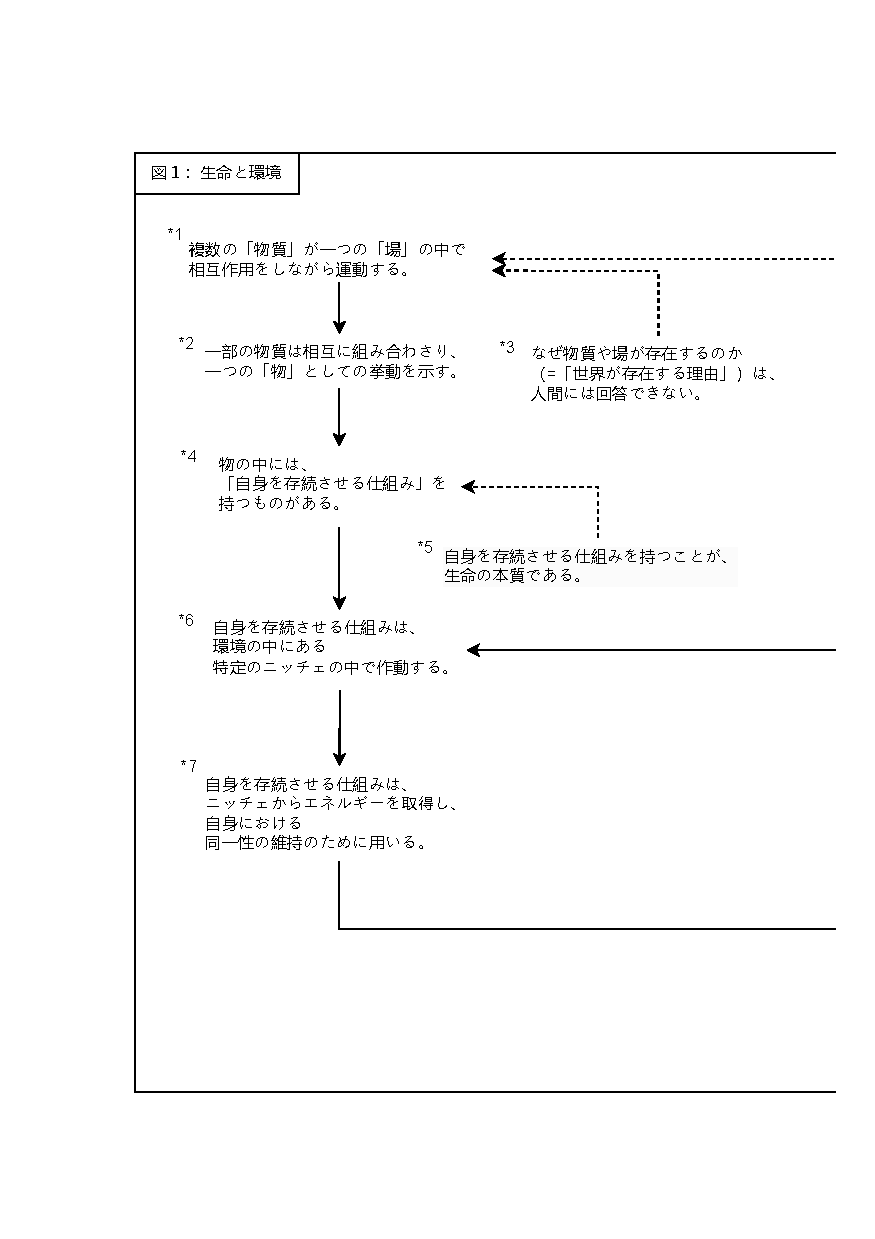
\includepdf[pages=-, scale=0.95, pagecommand={\thispagestyle{plain}}]{../figures/図1.pdf}

% Options for packages loaded elsewhere
\PassOptionsToPackage{unicode}{hyperref}
\PassOptionsToPackage{hyphens}{url}
%
\documentclass[
]{ltjsarticle}
\usepackage{amsmath,amssymb}
\usepackage{iftex}
\ifPDFTeX
  \usepackage[T1]{fontenc}
  \usepackage[utf8]{inputenc}
  \usepackage{textcomp} % provide euro and other symbols
\else % if luatex or xetex
  \usepackage{unicode-math} % this also loads fontspec
  \defaultfontfeatures{Scale=MatchLowercase}
  \defaultfontfeatures[\rmfamily]{Ligatures=TeX,Scale=1}
\fi
\usepackage{lmodern}
\ifPDFTeX\else
  % xetex/luatex font selection
\fi
% Use upquote if available, for straight quotes in verbatim environments
\IfFileExists{upquote.sty}{\usepackage{upquote}}{}
\IfFileExists{microtype.sty}{% use microtype if available
  \usepackage[]{microtype}
  \UseMicrotypeSet[protrusion]{basicmath} % disable protrusion for tt fonts
}{}
\makeatletter
\@ifundefined{KOMAClassName}{% if non-KOMA class
  \IfFileExists{parskip.sty}{%
    \usepackage{parskip}
  }{% else
    \setlength{\parindent}{0pt}
    \setlength{\parskip}{6pt plus 2pt minus 1pt}}
}{% if KOMA class
  \KOMAoptions{parskip=half}}
\makeatother
\usepackage{xcolor}
\setlength{\emergencystretch}{3em} % prevent overfull lines
\providecommand{\tightlist}{%
  \setlength{\itemsep}{0pt}\setlength{\parskip}{0pt}}
\setcounter{secnumdepth}{-\maxdimen} % remove section numbering
\usepackage{bookmark}
\IfFileExists{xurl.sty}{\usepackage{xurl}}{} % add URL line breaks if available
\urlstyle{same}
\hypersetup{
  hidelinks,
  pdfcreator={LaTeX via pandoc}}

\author{}
\date{}

\begin{document}

\section{細胞・遺伝情報・セントラルドグマ}\label{ux7d30ux80deux907aux4f1dux60c5ux5831ux30bbux30f3ux30c8ux30e9ux30ebux30c9ux30b0ux30de}

地球上の生命の身体は、細胞という単位からできている。細胞は「DNA(デオキシリボ核酸)」という化学物質を中に持っているが、そのDNAは四種類の「ヌクレオチド」という単純な化学物質が並んで結合することでできている。その四種類のヌクレオチドの配列パターンによって、その細胞がどのように「自身を存続させる仕組み」を作動させるかの大枠が決まる。具体的には、DNAをもとに「RNA(リボ核酸)」という化学物質が生成され(=「転写」)、そのRNAを元にタンパク質が生成される(=「翻訳」)。タンパク質は約20種類のアミノ酸という単純な化学物質が並んで結合してできており、生体内の様々な化学反応において触媒として作用する。つまり、生体内の化学反応を司るタンパク質がどのようなアミノ酸の配列パターンを持つかが、元を正せばDNAにおけるヌクレオチドの配列パターンによって決まっているわけだ。その意味で、DNAは生体内の化学反応を規定している。

細胞は自己複製を行って増殖するが、このとき、DNAが持つ配列パターンも「複製」され、細胞の複製に伴って細胞が行う生体内の化学反応のあり方も複製されることになる。こうした事情から、DNAが持つ配列パターンは「遺伝情報」と呼ばれる。遺伝情報の総体を「ゲノム」と呼ぶが、これは通常、細胞内に含まれるすべてのDNA分子の配列パターンの総体のことを指している。このようにして行われる遺伝情報の複製が、第一章の最後に述べた「同一性の維持」のための一つ目の仕組みだ(*1)。

ここまで述べてきたような「DNA→RNA→タンパク質」というゲノムから生体内の化学反応に至るまでの情報の流れと、「DNA→DNA」というゲノム自体の複製の流れを合わせて、「分子生物学のセントラルドグマ」という。地球上の生命は、基本的にセントラルドグマに沿った仕方で「自身を存続させる仕組み」を作動させている。なお、セントラルドグマに沿わない化学反応も存在している。例えば、「RNAの配列パターンに従ってDNAが作り出され(=『逆転写』)、そのDNAがある生物のDNAの中に挿入される」という現象もある。生命はニッチェとの相互作用の中から場当たり的に変化して生まれてきたものなので、単純な原理原則から逸脱する例外に満ちている。

\section{遺伝子と発現制御}\label{ux907aux4f1dux5b50ux3068ux767aux73feux5236ux5fa1}

このように書いたものの、生体内で合成されるタンパク質を構成するアミノ酸の配列パターンに対応しているのは、ゲノム中の配列パターンのうちの一部にすぎない。ゲノム中のタンパク質の配列パターンを直接規定している部分のことを、特に「遺伝子」と呼ぶ。

ゲノム中の遺伝子ではない部分は何をしているのかの全貌はまだ分かっていないが、その少なくない部分が「どのような条件下で、どの遺伝子からタンパク質を合成するか」を規定している。遺伝子からタンパク質が合成されることを、その遺伝子が「発現する」と表示し、そのタイミングなどを制御することを遺伝子の「発現制御」という。この発現制御が、生命に「変化」をもたらす二つの仕組みの一つだ(*3)。

遺伝子とその発現制御について理解すると、日常生活の様々なことについても納得しやすくなる。例えば、いわゆる「お酒に強いか否か」は、各個人がその細胞のうちに持つアルコールデヒドロゲナーゼというアルコールを分解するタンパク質に関わる遺伝子上の配列パターンに、その原因の大部分を求めることができると分かっている。また、「筋トレをすると筋肉量が増える」のは、筋トレにより細胞内でアクチンとミオシンという筋肉の伸縮に関わるタンパク質がより多く合成されるようになったり、筋繊維の外側に張り付いているサテライト細胞という細胞が増殖して筋繊維を増やすようになるからだということが分かってきている。

このように、遺伝子を含むゲノムだけで身体がどのようになるかが決まるわけではないし、育った環境だけでそれが決まるわけでもない。良く話題に上がる「生まれか育ちか」という議論の背後には、このような生物学的プロセスがある。

\section{突然変異と種}\label{ux7a81ux7136ux5909ux7570ux3068ux7a2e}

どの遺伝子がどのように発現するのかは細胞が置かれた状況によって規定されているわけだが、そもそも「アルコールデヒドロゲナーゼには、アルコールをよく分解できるものと、うまく分解できないものがある」といったDNAの配列パターンの多様性はどこから現れるのか。その原因は、DNAに損傷が入ったり、あるいはDNAが複製される際に正しく複製されなかったりすることで変異が入ること(=突然変異)に求められる(*4)。これが、生命に「変化」をもたらす二つの仕組みのもう一つだ。

ところで、通常では突然変異はすぐに修復される(*2)のだが、この突然変異が次の時代まで残留することもある。具体的には、細胞一つで「個体」として生きていくことが前提となっている単細胞生物(例えば、細菌)の場合では、ある個体に入った変異がそのまま分裂などによって多くの個体に増えていくことになるし、同一の遺伝情報を持った細胞が複数集まった状態で「個体」を形成して生きていくことが前提となっている多細胞生物(例えば、人間)の場合では、親個体に入った変異が子孫へと伝わっていくことになる。これらのプロセスを通じて、様々な遺伝情報を持つ個体が現れるようになる。

個体間の遺伝情報の違いが大きくなると、それらは互いに似た形態をしなくなっていったり、似た生態をとらなくなっていったり、あるいは近しい個体間で成立する関係性が成立しなくなったりする。最後に挙げた「近しい個体間で成立する関係性」の代表的な例が、「交配して子孫を残せるか、生まれた子孫は親同様に他の近しい個体と交配してさらなる子孫を残すことができるか」というものだ。例えば、イヌとネコの間には子供はできないし、雄のロバと雌のウマから生まれるラバは子供を残すことができない一代限りの動物だ。このような、ある程度の違いの幅を持った複数の類似した個体の集合を「種」という。なお、地球上の生命一般に対して「何をもって同じ『種』とみなすか」を規定する明確な統一的な見解は存在しない。

ここまでの議論で、生命が持つ「同一性の維持」と「変化」のための三つの仕組みについて、その概略を説明できた。生命は、基本的には同一性を維持する仕組みに従って生存していく。だが、ある個体から受け継がれる遺伝情報は、突然変異による時間的な揺らぎを受けていく。その揺らぎの結果として、ある個体たちと他の個体たちとの間に種の違いという境界線が生じてくることになる。その上、各個体はその生の中で発現制御を通じて周囲の環境から影響を受け、変化していく。これらの仕組みによって、生命は、その生命が生きるニッチェと共に、揺れ動く環境の中で変化していくのだ。

この議論を前提として、次章からは、「ある人間個体に対して、遺伝子の発現制御によって後天的な変化を与える仕組み」の一つである「脳」の振る舞いへと議論の対象をズームインしていく。脳は、その発達を通じて環境への特に繊細な適応を可能にする。この脳の振る舞いを見ていくことで、人間の思考がどのような制限下にあるのかの輪郭を浮き上がらせることができるだろう。

\section{種にとって寿命とは何か}\label{ux7a2eux306bux3068ux3063ux3066ux5bffux547dux3068ux306fux4f55ux304b}

だが、ここで第一章と同様に、視点を一度ズームアウトして「ある種にとって寿命とは何か」という問いについて考えておく。それは、そうすることが寿命を持つ種である人間を生きる私たちがいずれ死ぬ理由について考えることにもなるからだ{[}\^{}1{]}。

「種にとって寿命とは何か」を考えるために、寿命がない種を想定してみよう。寿命とは誕生後の時間経過と共に細胞の機能が低下していくことだと言えるので、ここではそうした機能低下が存在しないと前提してみる。すると、その種の個体は事故や病気以外では死亡しないことになる。このように想定すると、ここでは時間経過による細胞の機能低下が存在しないと想定しているので、年齢の低い世代からだけでなく、年齢の高い世代からも子孫が生まれることになる。この想定では、新しい時代に形成された遺伝情報だけからではなく、古い時代に形成された遺伝情報からも、新しい世代の遺伝情報が形成されることになる。そのため、種に新たに供給される遺伝情報は、現実世界のものと比べて、全体としてはより「古い」遺伝情報に偏ることになる。

これだけだと特に大きな問題にはならなさそうだが、ここに「ニッチェが許容する個体数の上限」を考慮の対象に追加すると、どうだろうか。ニッチェには許容する個体数に上限がある。例えば、種に供給される食料は、捕食される他の生物の量によって律速される。したがって、ある特定の種の個体数の上限値は寿命の長さにかかわらずそれほど変えられないということがわかる。この点を加味すると、寿命がない種では、寿命で死ぬ個体数が存在しない分だけ新たに出生する個体数が減っていなければならないことになる。さもなくば、その種は飢餓に見舞われてしまうだろう。

寿命がある場合と比較して「出生数が減り、さらに出生する新しい世代の遺伝情報がより『古い』ものに偏っている」となると、その種が持つ遺伝情報にもたらされる変化のスピードはより遅くなってしまう。新しい世代を生むのが仮に集団内の若い世代に限られる場合(つまり、生殖能力だけは老化すると仮定した場合)では、上記の事情は「出生数が減る」というだけなるので緩和されるが、その場合でも寿命がある場合よりは種の遺伝情報が変化するスピードは遅くならざるを得ない。

種の遺伝情報の変化速度が低下するということは、その種に属する個体の身体が変わる上限速度も低下するということを意味している。これは、急激な環境変動などに対応して身体を変化させることがより難しくなるという点で、生存に不利になる可能性がある。

ある種に寿命が存在することに上記のような背景があるのだとすれば、ここから翻って「寿命」と「世代交代」が、種の遺伝情報に変化を繰り込む手段の一つなのだと考えることができる(*5)。世代交代は新たな遺伝情報が種に組み込まれる機会なのであり(*6)、寿命が古い世代を排除することで、古い世代の遺伝情報が種から排除され、それが新たな遺伝情報が種に入り込む余地になるのだ(*7)。種の遺伝情報には流動性が繰り込まれており、その流動性が環境とニッチェの中での種の変形を可能にする。

人間が持つ寿命も、そうした種に流動性を繰り込む仕組みに起源を持つと考えられる。それゆえ、人類から寿命による死を遠ざけることには、ヒトという種の遺伝情報に変化を繰り込む機会を減少させることを意味するだろう。その場合、遺伝情報の変化という観点からみれば、ヒトはより硬直した、環境とニッチェの変化に対して脆弱な存在になる可能性が考えられる。

もちろん、「世界がどのようになっているか」という事実は「人がどのように生きるべきか」という当為を一切導かない。また、ここでも第一章と同様に、技術的な工夫が隘路を切り開く可能性は否定できない。それでも、この事実を認識することで、それに逆らうことにいかなる困難が伴うのかを明確に認識できるようになる。このような困難についての認識は、私たちが自らの生き方を構想し、また世界についての納得できる物語を作り上げる際に、野放図に空想が膨らむのを避ける役に立つことだろう。

\begin{itemize}
\tightlist
\item
  {[}\^{}1{]}
  以下の議論については主に小林武彦『生物はなぜ死ぬのか』を参考にした。
\end{itemize}

\end{document}

\newpage
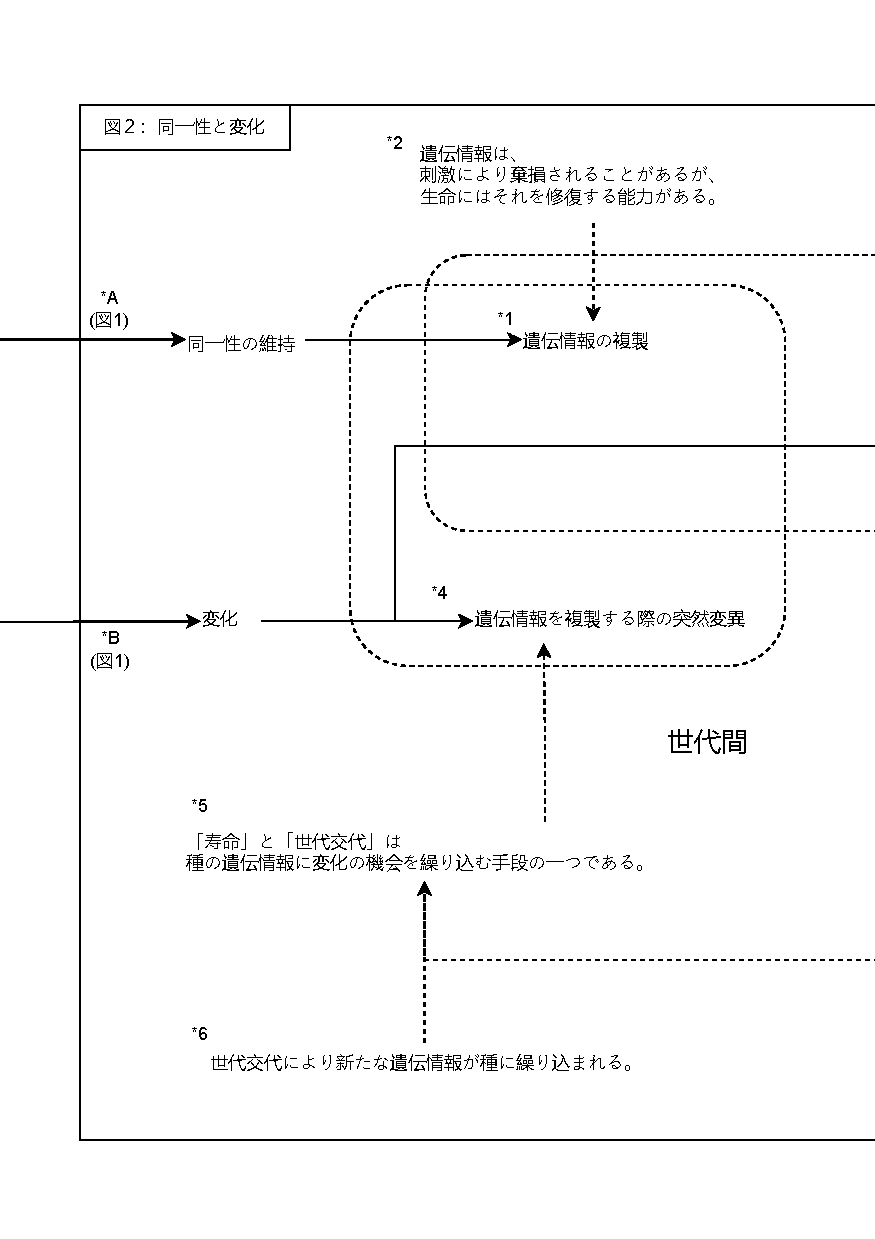
\includepdf[pages=-, scale=0.95, pagecommand={\thispagestyle{plain}}]{../figures/図2.pdf}

\section{第三章:脳と自由エネルギー原理}\label{ux7b2cux4e09ux7ae0ux8133ux3068ux81eaux7531ux30a8ux30cdux30ebux30aeux30fcux539fux7406}

\subsection{脳・学習・最適化}\label{ux8133ux5b66ux7fd2ux6700ux9069ux5316}

多細胞生物の一部には、身体の様々な箇所で起きた出来事について、その情報をまとめた上でそこから全身を適切に動かすための「神経」がある。多くの神経が集まる場所には特に多くの情報が集まり、より統合的な情報処理が行われる。どれくらいの神経がどのように集まるかは生物によりさまざまだ。例えば、昆虫ではその頭部から尾部にかけて「はしご形」に神経が走っており、そのはしご形に走っている神経の頭部以外にも数か所、神経細胞が多く集まっている場所がある。

人間を含む一部の生物に備わるそうした神経細胞の集まりは「脳」と呼ばれる。脳は、外界からの入力に応じて行動を制御する神経網である(*1)。例えば、人間の網膜は二次元上の視覚情報を受け取るが、その情報は脳で様々に分析され、目の前に何が存在しているかが判断される{[}\^{}1{]}。そして、その判断はさらに脳での情報処理を経て、その後に取られる行動に影響を及ぼす。なお、すべての行動が脳による判断に従っているわけではない。実際、内部で水を沸騰させているやかんなどに手で触れてしまった場合、熱いものに触れたという情報が手から脊髄へと伝わるが、脊髄から脳へと情報が伝わるまでもなく、脊髄から腕へと筋肉を収縮されて手を引っ込めるための電気刺激による指令が出る。このような反射に用いられる脳を介さない神経の経路を「反射弓」という。

多くの「脳」は、環境との相互作用を通じて後天的かつ柔軟に変化する(*2)。この後天的な変化は「学習」と呼ばれるが、脳を持つ生物は学習によって遺伝情報というハード面での変化を待つことなく身体の使い方というソフト面を変えることができる。それゆえに、学習は身体が許容する範囲で自らを取り巻く環境との関係性を素早く最適化することができるわけだ。

人間が構築してきた思考や社会もそうした学習による最適化の産物だと言える。そのため、学習と最適化がどのようにして行われるのかを理解することで、人間の思考や社会の成り立ちや構造、そして限界を理解することができる。それゆえに、この章では脳の振る舞いを理解することで、学習や最適化の仕組みを理解することを目指す。

\begin{itemize}
\tightlist
\item
  {[}\^{}1{]}
  乾敏郎・坂口豊『脳の大統一理論―自由エネルギー原理とはなにか』p.1-3,9-10を参照。
\end{itemize}

\subsection{感覚信号・予測信号・予測誤差}\label{ux611fux899aux4fe1ux53f7ux4e88ux6e2cux4fe1ux53f7ux4e88ux6e2cux8aa4ux5dee}

本稿では、2006年頃からイギリスの研究者であるカール・フリストン(1959~)によって提唱されるようになった「自由エネルギー原理」(*3)にしたがって、脳の振る舞いを説明していく{[}\^{}1{]}。自由エネルギー原理において、「脳はヘルムホルツの自由エネルギーを最小化するように推論を行う」とされているが{[}\^{}2{]}、これは具体的には脳が「予測誤差」を最小化するように動作することに等しい(*4){[}\^{}3{]}。

まず、脳の仕事とは、脳が受け取った感覚信号 \(s\) から外界の真の状態
\(u\) を推論することである。そのために、脳は「外界が状態 \(u_i\)
を取っていると想定」した上で、「その想定が正しかった場合に外界から受け取るはずの予測信号
\(g(u_i)\) 」と計算する能力を持つ。こうすると、脳は感覚信号 \(s\)
と予測信号 \(g(u_i)\) の差分 \(s-g(u_i)\) から、自身の想定 \(u_i\)
がどれほど間違っていたかを測定することができる。この感覚信号 \(s\)
と予測信号 \(g(u_i)\) の差分 \(s-g(u_i)\)
が予測誤差だ(*5)。脳の仕事は外界の真の状態 \(u\)
を求めることであるので、そのために脳は予測誤差 \(s-g(u_i)\)
をより少なくする新たな外界についての想定 \(u_{i+1}\)
を求めればよいことになる{[}\^{}4{]}。

なお、脳は予測誤差をどれだけ重大に捉えるか(=「精度」)を自主的に制御することができる。例えば、わずかな予測誤差であっても高い精度を求めて受け取るのであれば、それは重大な想定の欠陥を表すものであると認識されて想定を更新しなおすことになるのに対し、逆に大きな予測誤差であっても求める精度が低いのであれば、それは些細な誤差として想定の更新を引き起こさないことになる。この精度の制御が「注意」えある(*7,
8){[}\^{}5{]}。

\begin{itemize}
\tightlist
\item
  {[}\^{}1{]}
  乾敏郎・坂口豊『脳の大統一理論―自由エネルギー原理とはなにか』ivを参照。
\item
  {[}\^{}2{]} 同、p.4を参照。
\item
  {[}\^{}3{]} 同、p.16-24を参照。
\item
  {[}\^{}4{]} 同、p.18を参照。
\item
  {[}\^{}5{]} 同、p.25-33を参照。
\end{itemize}

\subsection{自由エネルギー原理・ダイバージェンス}\label{ux81eaux7531ux30a8ux30cdux30ebux30aeux30fcux539fux7406ux30c0ux30a4ux30d0ux30fcux30b8ux30a7ux30f3ux30b9}

予測誤差の最小化は、下記の式の「変分自由エネルギー」の最小化と等価である(*6){[}\^{}1{]}。変分自由エネルギーは、下記の式で表される:
\[
(変分自由エネルギー)=(ダイバージェンス)+(シャノンサプライズ)\tag{1}
\]
この式について説明するため、具体例として東京に2023年から住むようになり、あまりの暑さから東京での8月の最高気温を気にするようになった人のことを考える。その人は、毎日晴れたり曇ったりする天候と共に、最高気温の高い日や低い日を経験する。このとき、この人は\textbf{毎日の最高気温を感覚信号の列
\(s\) として受け取っている}ということになる。

さて、この感覚信号の列 \(s\)
は、地球と宇宙の極めて複雑な依存関係によって生成されるわけだが、そのプロセスの全貌は不可知であり、かつ普通に生きる人にとっては(少なくとも当面は)関心の対象にならない{[}\^{}2{]}。普通の人にとって関心があるのは、受け取った感覚信号の列
\(s\)
を生成した外界の状態を正しく反映した式だ{[}\^{}3{]}。つまり、その人は
\textbf{「東京の8月の最高気温は、 \(x_1\) \%で \(t_1\) 度、 \(x_2\) \%で
\(t_2\) 度\ldots\ldots{} \(x_n\) \%で \(t_n\)
度を取る」といったような、東京における8月の最高気温についての確率分布
\(p(u)\)} に関心があるわけだ。

その確率分布 \(p(u)\)
を求めるために、この人は最初に2023年8月の東京として表1のような感覚信号の列
\(s_0\)
を経験する。すると、2023年9月1日時点でのその人にとっての外界の状態を表す確率分布
\(p(u_0)\)
は(最初の年は極めて素朴に頻度からそのまま確率分布を考えたと前提すれば)表2のようになる。そして次の年、その人は2024年も8月を東京で過ごして表3のような感覚信号の列
\(s_1\) を経験する{[}\^{}4{]}。

\[
\begin{array}{cc}
~~~\textrm{最高気温(℃)}~~~ & ~~~\textrm{日数}~~~ \\
\hline
\textrm{31} & \textrm{1} \\
\textrm{32} & \textrm{6} \\
\textrm{33} & \textrm{2} \\
\textrm{34} & \textrm{13} \\
\textrm{35} & \textrm{8} \\
\textrm{36} & \textrm{1}
\end{array}
\tag{表1}
\]

\[
\begin{array}{cc}
~~~\textrm{最高気温(℃)}~~~ & ~~~\textrm{確率}~~~ \\
\hline
\textrm{31} & \textrm{3.26\%} \\
\textrm{32} & \textrm{19.4\%} \\
\textrm{33} & \textrm{6.45\%} \\
\textrm{34} & \textrm{41.9\%} \\
\textrm{35} & \textrm{25.8\%} \\
\textrm{36} & \textrm{3.26\%}
\end{array}
\tag{表2}
\]

\[
\begin{array}{cc}
~~~\textrm{最高気温(℃)}~~~ & ~~~\textrm{日数}~~~ \\
\hline
\textrm{27} & \textrm{1} \\
\textrm{29} & \textrm{1} \\
\textrm{30} & \textrm{1} \\
\textrm{31} & \textrm{4} \\
\textrm{32} & \textrm{1} \\
\textrm{33} & \textrm{7} \\
\textrm{34} & \textrm{9} \\
\textrm{35} & \textrm{7}
\end{array}
\tag{表3}
\]

いま、確率分布 \(p(u_0)\) を、感覚信号の列 \(s_1\)
を用いて新しい確率分布 \(p(u_1)\)
に更新することを考える。この新しい確率分布 \(p(u_1)\)
は、ベイズ推定という確率論の考え方を用いて事後確率分布 \(p(u|s)\)
として表現できる。したがって、その人の\textbf{脳が解くべきタスクは、外界
\(u\) がとる状態の確率分布 \(p(u)\)
を知るために、ある時点までに考えていた(事前)確率分布 \(p(u_i)\)
と、新たに得られた感覚信号の列 \(s_{i+1}\)
を用いて、更新された(事後)確率分布 \(p(u|s_{i+1})\)
」を知ること}となる{[}\^{}5{]}。

この \(p(u|s_{i+1})\)
を自由エネルギー原理の文脈では「真の事後確率分布」という。「真の」と銘打ってはいるものの、この確率分布は感覚信号の列
\(s\)
から計算可能な外界についての暫定的な理解を表すものであり、それゆえ暗黙的・潜在的に与えられているというのがポイントだ。例えば、いま考えている東京で8月の最高気温を気にする人の場合、(\(s_0\)
について27度から36度の範囲でラプラス・スムージングすることで \(p(u_0)\)
を補正した上で、尤度計算の際に正規分布の確率密度関数を用いたと前提すれば)2024年9月1日時点での真の事後確率分布
\(p(u|s_1)\) は表4のようになる。

\[
\begin{array}{cc}
~~~\textrm{最高気温(℃)}~~~ & ~~~\textrm{確率}~~~ \\
\hline
\textrm{27} & \textrm{0.03\%} \\
\textrm{28} & \textrm{0.11\%} \\
\textrm{29} & \textrm{0.39\%} \\
\textrm{30} & \textrm{1.00\%} \\
\textrm{31} & \textrm{3.96\%} \\
\textrm{32} & \textrm{21.0\%} \\
\textrm{33} & \textrm{10.4\%} \\
\textrm{34} & \textrm{42.6\%} \\
\textrm{35} & \textrm{18.5\%} \\
\textrm{36} & \textrm{2.11\%}
\end{array}
\tag{表4}
\]

このように、真の事後確率分布 \(p(u|s_1)\)
を知るためには、ここで扱っているような簡単な例ですら、かなりしっかりとした計算が必要となる。上段で「(理念的には)計算できる」や「暗黙的・潜在的に与えられている」などといった歯切れの悪い表現をしていたのは、その計算が多くの場合で事実上不可能だということを示すためだ。複雑な事例に囲まれた実生活においては、真の事後確率分布は計算できない場合が多いだろう。

そのため、日々の最高気温を気にするだけの普通の人が持つ外界についての認識は、もっと簡単なものに留まる。例えば、その認識は「東京では、8月の最高気温は概ね30度より高い。35度より暑くなることもままある」という程度のものだろう。重要なのは、それくらいの認識でも生存には十分に役立つということだ。この
\textbf{真の事後確率分布 \(p(u|s_{i+1})\)
の近似として使う「外界がとる状態についての確率論的な認識」を「認識確率分布
\(q(u_{i+1})\) 」と表現する} {[}\^{}6{]}。

ここで、認識確率分布 \(q(u_1\)) と真の事後確率分布 \(p(u|s_1)\)
との違いを確率論の言葉で表現したものが上述の式における「(カルバック・ライブラー)ダイバージェンス」だ(*9){[}\^{}7{]}。このダイバージェンスを計算する式は下記のようになっている:
\[
(ダイバージェンス)=(変分自由エネルギー)-(シャノンサプライズ)\tag{2}
\] それゆえに、この節の冒頭の式 (1)
で表したように変分自由エネルギーを記述できるわけだ{[}\^{}9{]}。なお、シャノンサプライズは、感覚信号の列
\(s_{i+1}\) が観測される確率 \(p(s_{i+1})\)
の対数の符号を反転させたものとして定義されるもので、その感覚信号の列が与えられることが稀であるほど大きな値をとる(*10)。

\begin{itemize}
\tightlist
\item
  {[}\^{}1{]}
  乾敏郎・坂口豊『脳の大統一理論―自由エネルギー原理とはなにか』p.21-22を参照。
\item
  {[}\^{}2{]} 同、付録p.11を参照。
\item
  {[}\^{}3{]} 同、付録p.8を参照。
\item
  {[}\^{}4{]}
  気象庁「気象庁|過去の気象データ検索」(\url{https://www.data.jma.go.jp/obd/stats/etrn/view/daily_h1.php?prec_no=44&block_no=00&year=2023&month=08&day=&view=p3})(2024年9月12日取得)を参照。
\item
  {[}\^{}5{]}
  乾敏郎・坂口豊『脳の大統一理論―自由エネルギー原理とはなにか』p.10-12およびp.19-20を参照。
\item
  {[}\^{}6{]} 同、p.21および付録p.7-8を参照。
\item
  {[}\^{}7{]} 同、付録p.7-9を参照。
\item
  {[}\^{}8{]} 同、p.114を参照。
\item
  {[}\^{}9{]} 同、付録p.9を参照。
\end{itemize}

\subsection{信念の更新・運動}\label{ux4fe1ux5ff5ux306eux66f4ux65b0ux904bux52d5}

式 (1)
から分かる通り、変分自由エネルギーを小さくするためには二つの方法がある。それは、ダイバージェンスを小さくする方法と、シャノンサプライズを小さくする方法だ。自由エネルギー原理においては、脳はこの二つを実現する機能を備えていると考えられている。では、この二つの方法について順にみていこう。

まず、ダイバージェンスを小さくする方法についてだ。この方法では、脳内で認識確率分布
\(q(u)\)
について「勾配降下法」と見なすことができる計算が行われ、ダイバージェンスの最小化が図られるとされている(*11){[}\^{}1{]}。勾配降下法とは、求める評価値(ここではダイバージェンス)がそれ以上下がらなくなるまで、少しずつ関数(ここでは認識確率分布
\(q(u)\) )を変化させていくことによって、求める関数(
ここでは真の事後確率分布 \(p(u|s)\)
)へと操作する関数を近づけていく計算手法である。このような方法を用いて、認識確率分布を更新する行為を、自由エネルギー原理では「無意識的推定」という(=「信念の更新」)(*12){[}\^{}2{]}。

もう一つが、シャノンサプライズを小さくする方法だ。その方法では、脳は認識確率分布
\(q(u_i)\) は変動させずに、シャノンサプライズ \(-\log{p(s_{i+1})}\)
が低くなるように、観測される確率が高い感覚信号の列 \(s_{i+1}\)
を狙って獲得しようとする(*16)。もし、その試みが成功すれば、それはその時点で採用している外界についての想定
\(u_i\)
が正しいことの証拠になる(*14){[}\^{}3{]}。つまり、脳は外界のサンプリングを通じて自分の推定が正しいことの証拠を能動的に集めているのであり、このような能動的なサンプリングを通じて脳は「自己証明」しているのだ(=「能動的推論」)(*15){[}\^{}4{]}。

このような「認識確率分布 \(q(u_i)\) を変えずに、得られる感覚信号の列
\(s_{i+1}\)
の側を変える」という行為を実現する仕組みが「(身体の)運動」だ。身体の運動を司る大脳の一部分を運動野と呼ぶが、運動野からは「運動するとこのような筋感覚信号が観測されるはずだ」という「筋感覚の予測信号」が出力される。すると、それが反射弓に伝わって筋収縮を起こし、身体が動く。そして、反射弓では「α運動ニューロン」という神経細胞が筋感覚の予測信号に合致するように筋肉が制御される(*13){[}\^{}5{]}。この一連の過程において認識確率分布
\(q(u_i)\)
が更新されないのは、運動野などの運動皮質には大脳皮質外からの入力信号が入ってくる第Ⅳ層という部分がほとんど見られないことから、感覚フィードバックの影響を受けないからだと考えられている{[}\^{}6{]}。

\begin{itemize}
\tightlist
\item
  {[}\^{}1{]}
  乾敏郎・坂口豊『脳の大統一理論―自由エネルギー原理とはなにか』付録p.14を参照。
\item
  {[}\^{}2{]} 同、p.2-3および付録p.9-10を参照。
\item
  {[}\^{}3{]} 同、付録p.11を参照。
\item
  {[}\^{}4{]} 同、p.24を参照。
\item
  {[}\^{}5{]} 同、p.35-45を参照。
\item
  {[}\^{}6{]} 同、p.46-47を参照。
\end{itemize}

\subsection{自由エネルギー原理から差異に開かれた弁証法へ}\label{ux81eaux7531ux30a8ux30cdux30ebux30aeux30fcux539fux7406ux304bux3089ux5deeux7570ux306bux958bux304bux308cux305fux5f01ux8a3cux6cd5ux3078}

さて、ここまで自由エネルギー原理に基づいて統一的に見てきた脳の振る舞いを、「脳と外界との間でなされる弁証法」として解釈しなおすことにしよう。なお、本稿では「ある存在(正)が、その存在を否定する物事(反)に出会うことで、変化する(合)」ようなプロセスとして弁証法を理解することにする。そうすることで、ここから先の議論を「見通しが良く、十分に自由だが適切に制限された視座」から統一的に把握できるようになるからだ。本稿がここまで「(いわゆる)理系」的な科学的知見をおさらいしてきたのは、そうした視座を得るためだった。

弁証法のプロセスとして脳の振る舞いを考えるとき、自由エネルギー原理では予測誤差の最小化が図られているのだから、そのプロセスは予測信号と感覚信号との間から起こると言える。つまり、脳が持つ外界についての信念をモデルとして、そのモデルに基づいた未来についての予期がなされ、それが予測信号として発せられる。そこに外界から入ってきた感覚信号が照らし合わされ、両者の間にある差異が予測誤差として発生する。そして、予測誤差を最小化する二つの方法に対応して信念の更新や身体の運動が起こるわけだが、この予測誤差の最小化が弁証法における正と反から合が作られる段階に相当していると考えられるだろう。その一方である信念の更新においては、予測誤差を最小化するような予測信号を生成できる信念が合として作り出される。また他方である身体の運動においては、正としての自身の信念に対して、それにそぐわない感覚信号としての反が得られないことを確認することにより、信念がより確証の深まったものとしての合になる。

このような構図から弁証法についての理解を更新することで、弁証法にまつわる様々な概念についても理解を改め、今後の章での見通しを良くすることができる。本稿が更新の対象として念頭に置いているのは、20世紀後半のいわゆるフランス現代思想における弁証法に対する理解だ。そこでは、弁証法を「世界のあらゆるところに差異を見出しつつも、それらを真なる世界の本質から生じた見せかけ上の対立だと見なす」発想に基づいたものだと見なした上で、その発想からは「あらゆるものの背後に理想が見出され、現に存在している多様な差異が抑圧されてしまう」とされてきた。そのため、フランス現代思想は「差異を肯定し、解放する」ことを提唱してきた。こうした弁証法に対する批判的な態度の背景には、西洋近代思想が「本当の〇〇(例えば、本当の『ドイツ人』)」といった理想を様々な対象の背後に見出し、その理想から逸脱するもの(例えば、「ユダヤ人」)に対して有形無形の暴力を振るってきたことの反省があった{[}\^{}1{]}。

しかし、このような弁証法理解は、少なくとも本稿が自由エネルギー原理に沿って考える弁証法に対しての理解とは合致しない。まず、本稿が考える弁証法においては、真なる世界の本質はたしかに予測誤差の最小化という形で目指されるものの、それが脳に与えられることはない。なぜならば、真なる世界の本質に向かうための手段として脳が使用できるのは変分ベイズ推論でしかないため、予測誤差を最小化できる信念は「場当たり的・発見的に作られる」しかないからだ。つまり、真なる世界の本質は、永遠不変の原理原則から導出されるようなものではなく、そこに向かって彷徨い歩くようにして近づいていくしかないものなのだ。

たしかに、普遍的な科学法則などについては人間の知は宇宙の様々な現象を説明できる域にまで達するかもしれない。だが、それでも人間の知は、具体的な個別の状況については、依然として無に等しいままに留まる他ない。何故ならば、そもそも量子力学の知見からして、厳密に対象の状態について知ることは不可能であり、よしんば対象の状態について厳密に知ることができたとしても、その対象がどのように変わっていくかの予測は確率的なものとならざるを得ないからだ。その上さらに、決定論的なシステムを対象に未来を予測しようとした場合ですら、三体問題のように任意の時間が経過した後の状態をピタリと計算することが不可能なシステムで世の中は満ちている。

だから、予測誤差は最小化を目指されるに過ぎず、それがゼロになることは決してありえない。ある生物が、具体的な物事についてその未来を正確に知ることはありえないわけだ。そのため、脳が思い描く理想というのはどこまでいっても曖昧で実現可能性に疑問符が付く無責任なものでしかない。ゆえに、生物が何らかの物事に対してそれを「善導」できるような立場に立つこともないのだ。

このように、脳は予測誤差がゼロにならない状況から逃れることはできない。そのような状況下で現前した予測誤差を受け入れないことは、単なる現状否認であり、弁証法の停止でしかない。脳は未来を予期し、能動的推論としての運動に際しては未来に対して目的を立てて能動的に行動することを可能にする。しかし、その結末は常に未知の差異に対して開かれているのだ。この「差異に開かれた、予測誤差の最小化を目指して弁証法的に変わりし続ける脳」という観点が、先に述べた、ここから先の議論を統一的に把握するのに役立つ「見通しが良く、十分に自由だが適切に制限された視座」だ。

{[}\^{}1{]} 小坂修平『図解雑学現代思想』を参照。

\newpage
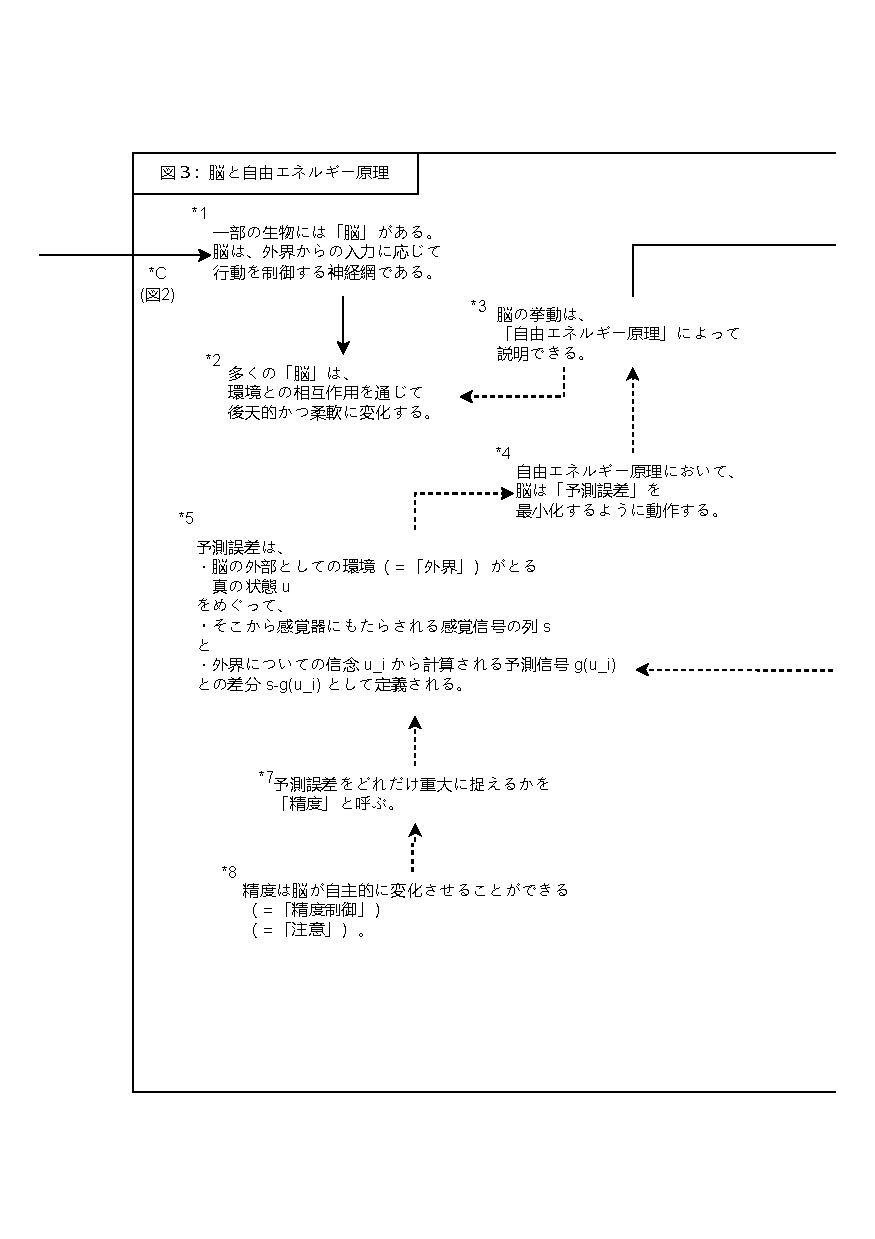
\includepdf[pages=-, scale=0.95, pagecommand={\thispagestyle{plain}}]{../figures/図3.pdf}

\section{第二部:体験とシニフィアンとの弁証法が形成する準安定状態としての四つのディスクール}

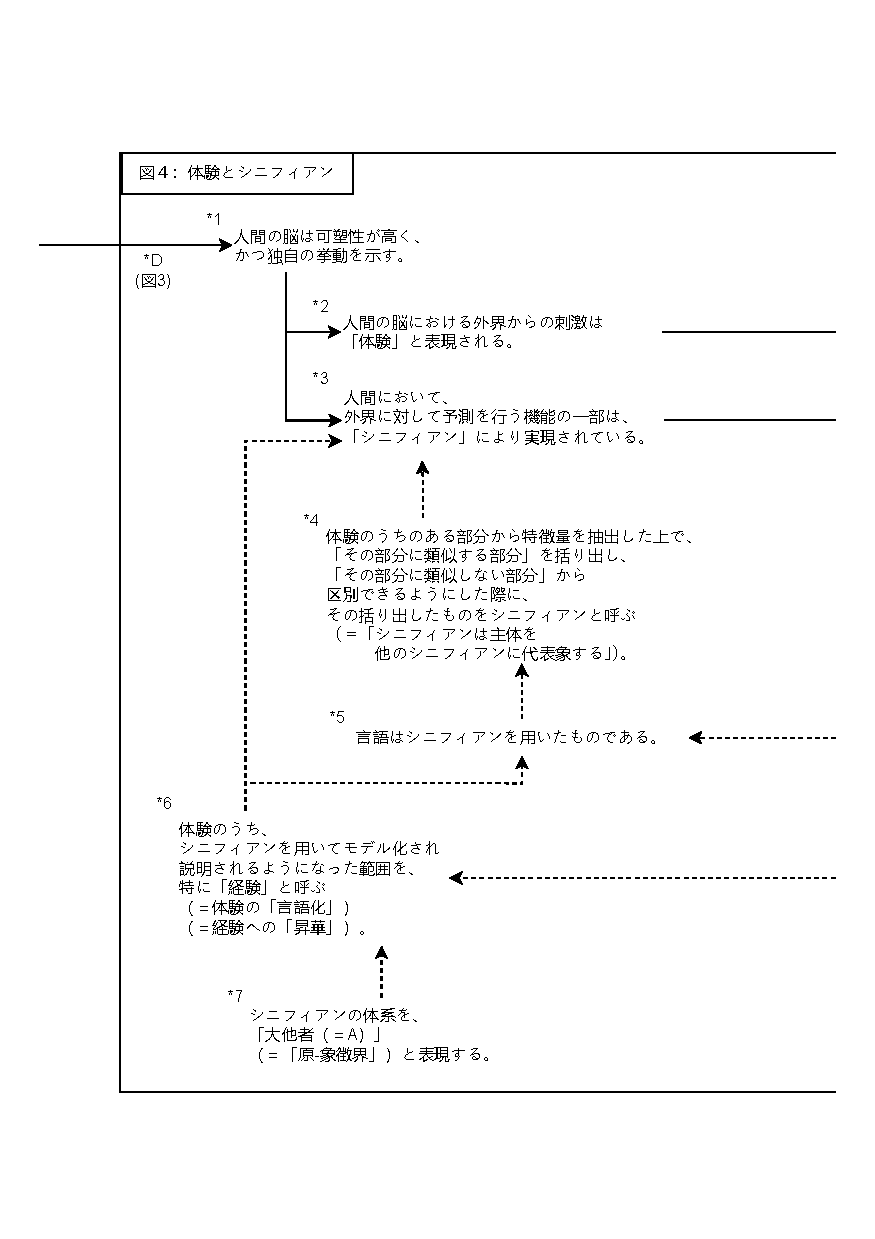
\includepdf[pages=-, scale=0.95, pagecommand={\thispagestyle{plain}}]{../figures/図4.pdf}

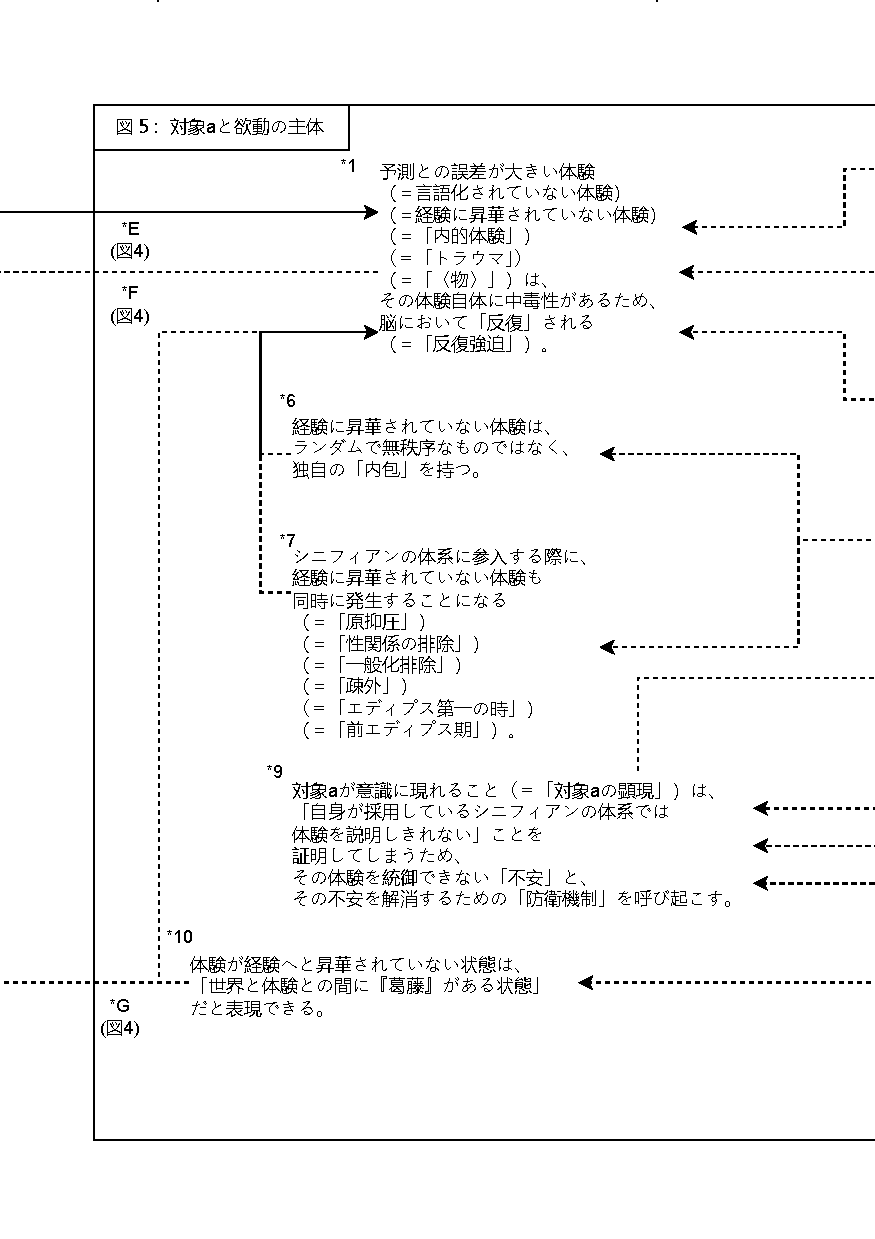
\includepdf[pages=-, scale=0.95, pagecommand={\thispagestyle{plain}}]{../figures/図5.pdf}

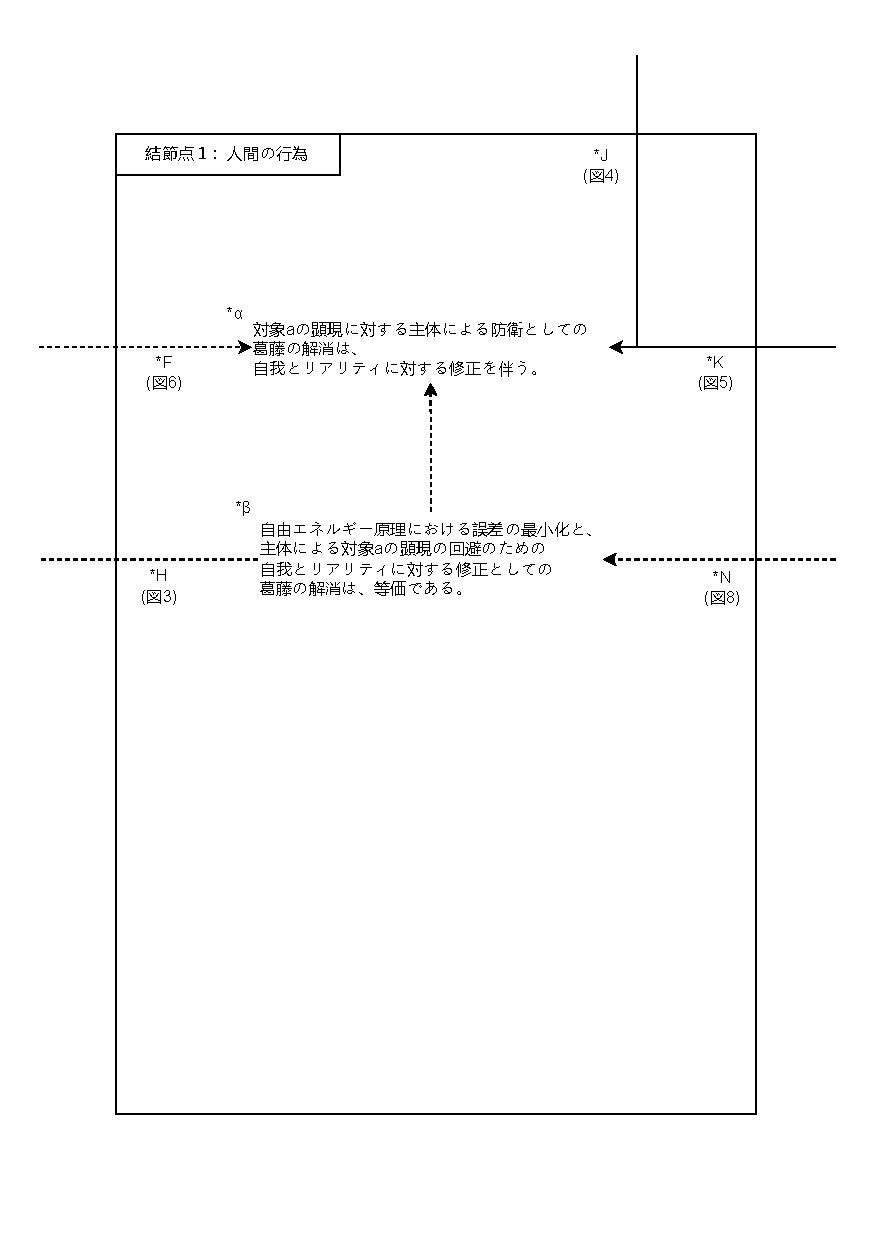
\includepdf[pages=-, scale=0.95, pagecommand={\thispagestyle{plain}}]{../figures/結節点1.pdf}

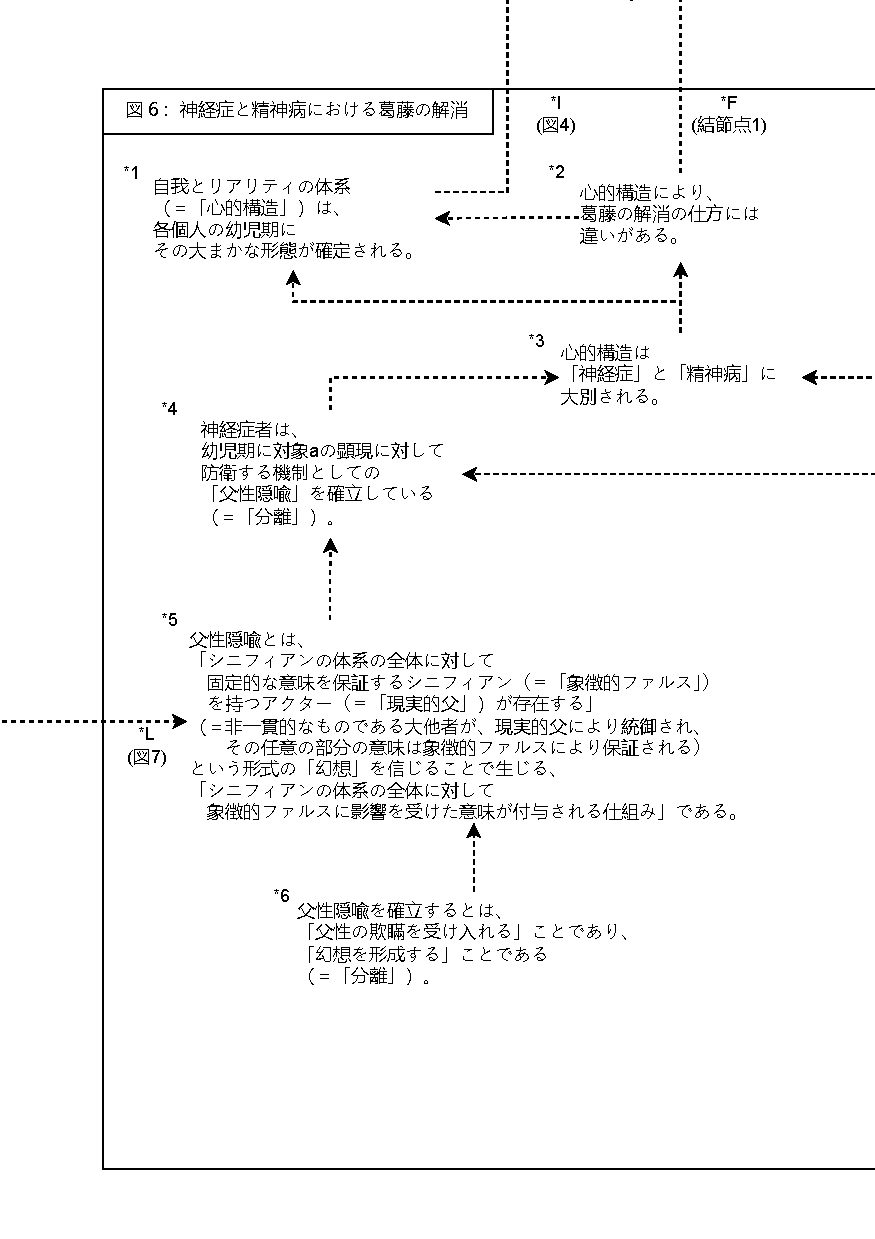
\includepdf[pages=-, scale=0.90, pagecommand={\thispagestyle{plain}}]{../figures/図6.pdf}

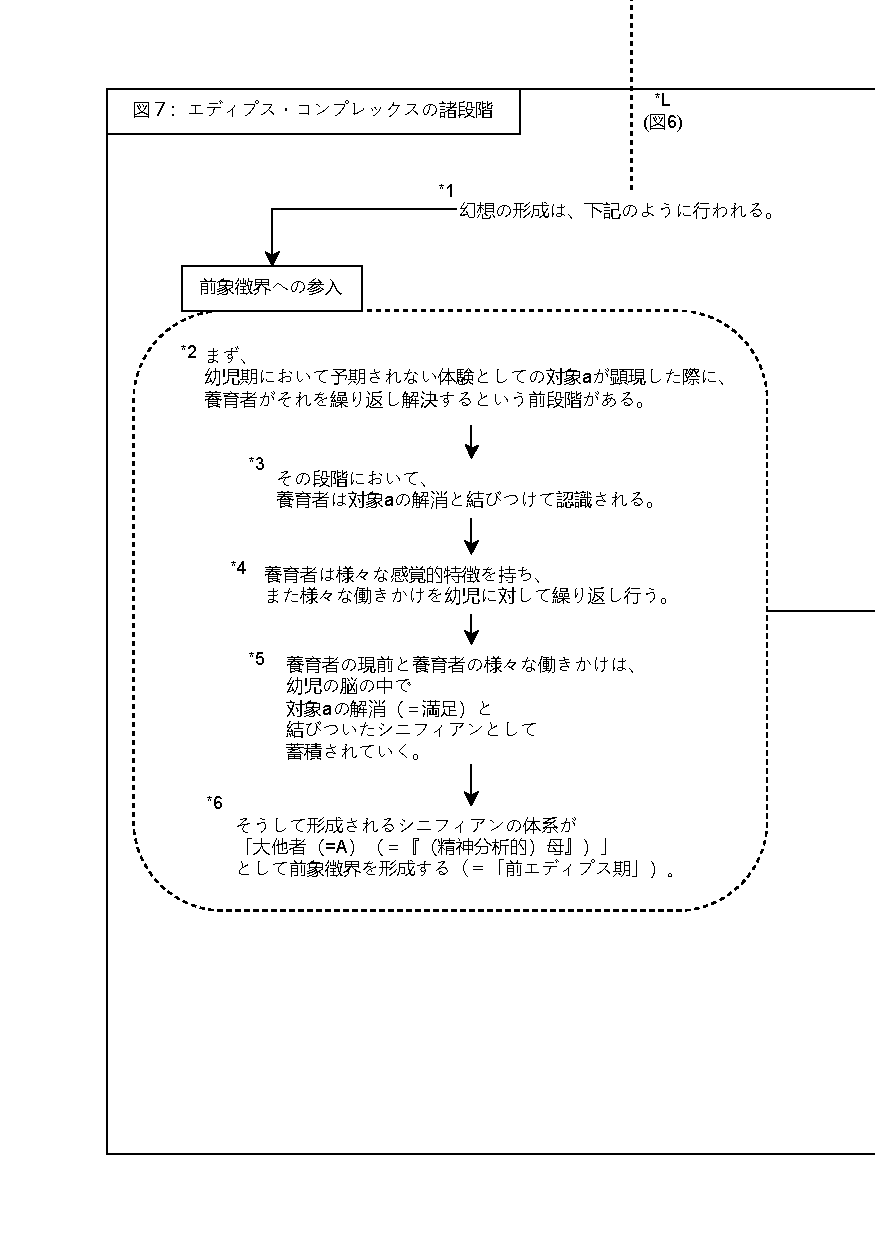
\includepdf[pages=-, scale=0.90, pagecommand={\thispagestyle{plain}}]{../figures/図7.pdf}

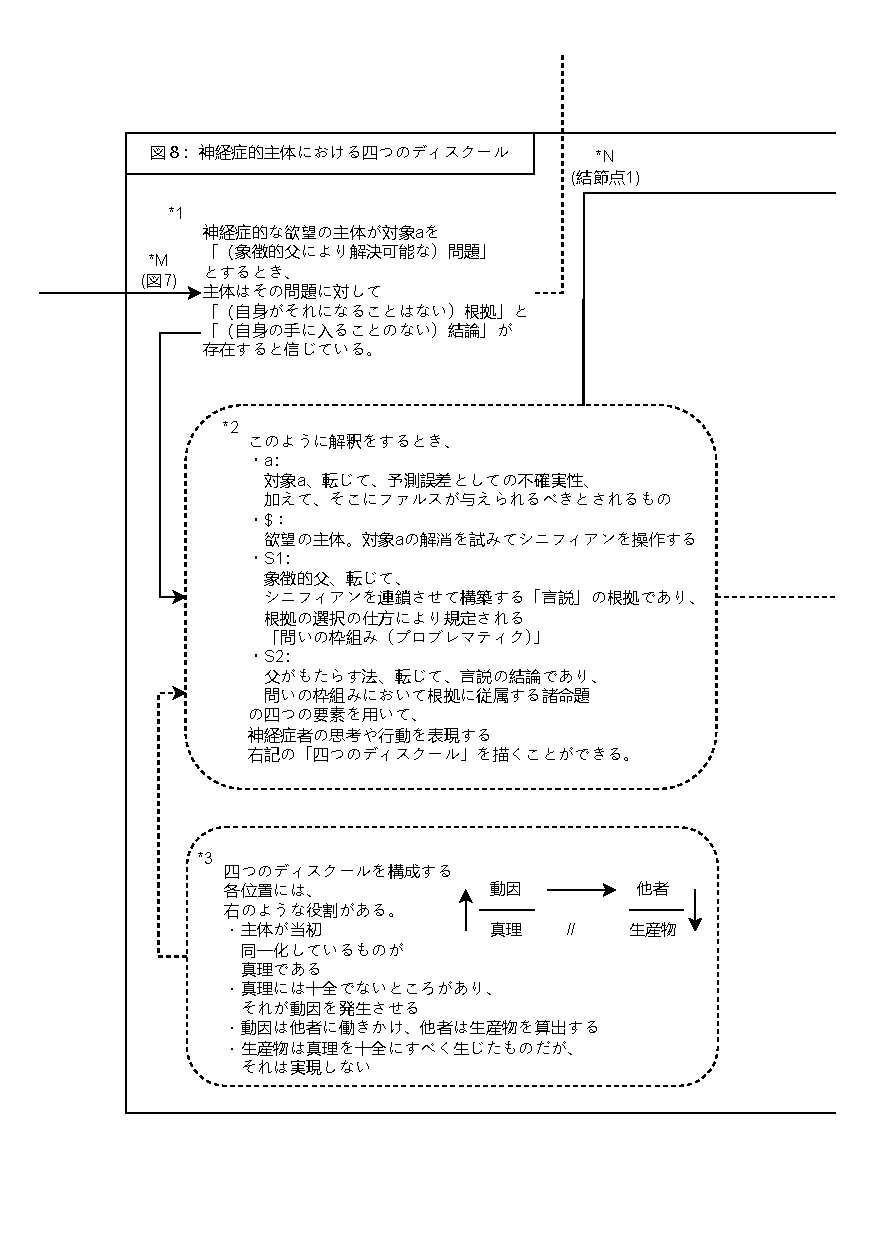
\includepdf[pages=-, scale=0.90, pagecommand={\thispagestyle{plain}}]{../figures/図8.pdf}

\section{第三部:四つのディスクールが形成する人間社会のダイナミズム}

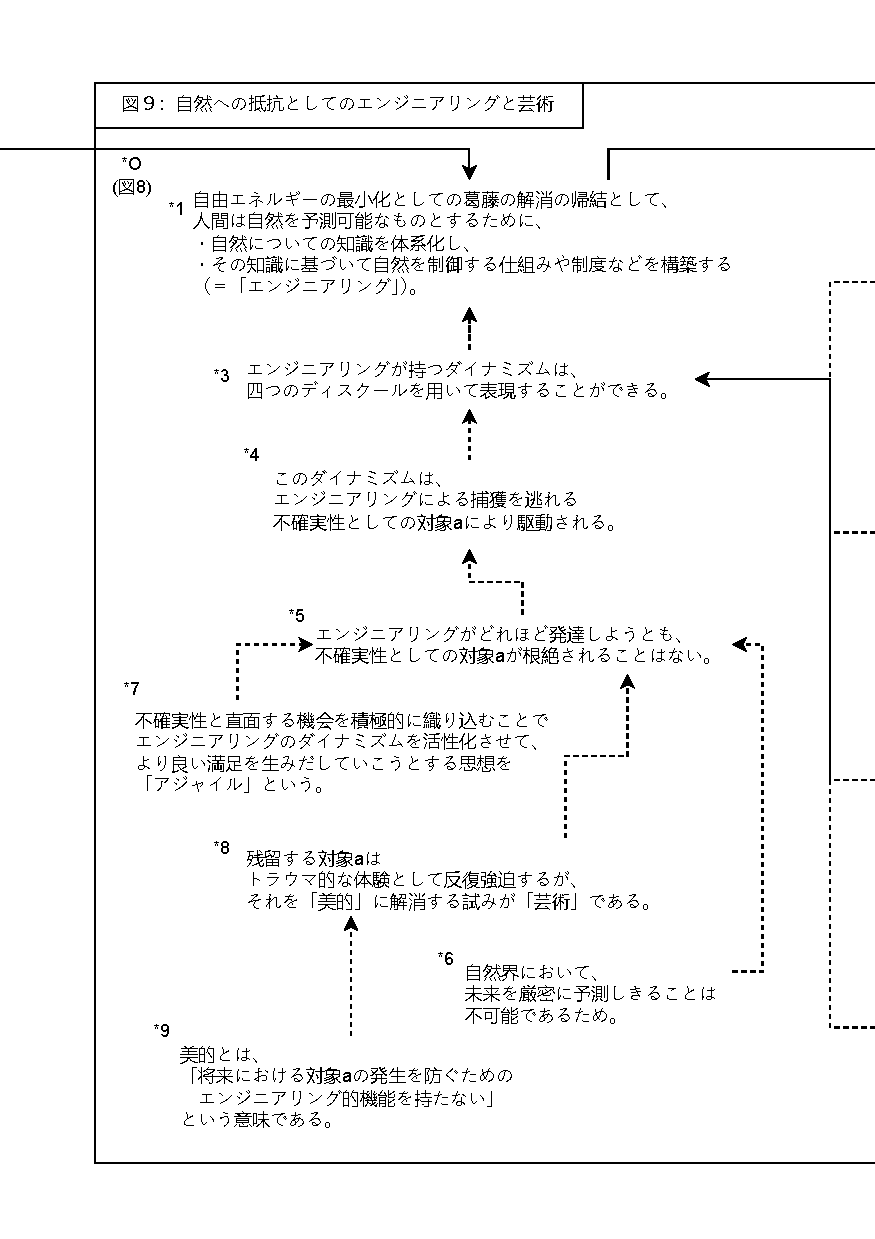
\includepdf[pages=-, scale=0.90, pagecommand={\thispagestyle{plain}}]{../figures/図9.pdf}

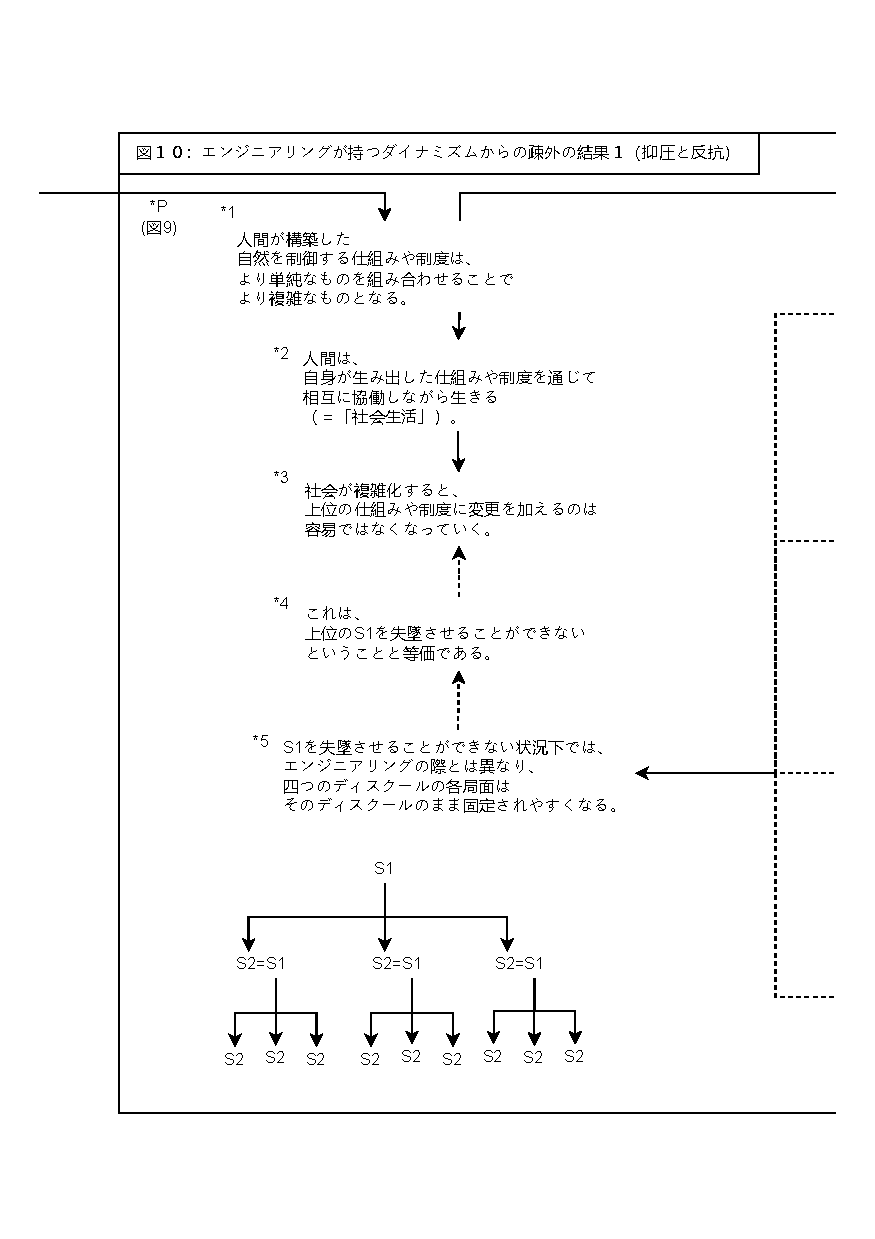
\includepdf[pages=-, scale=0.90, pagecommand={\thispagestyle{plain}}]{../figures/図10.pdf}

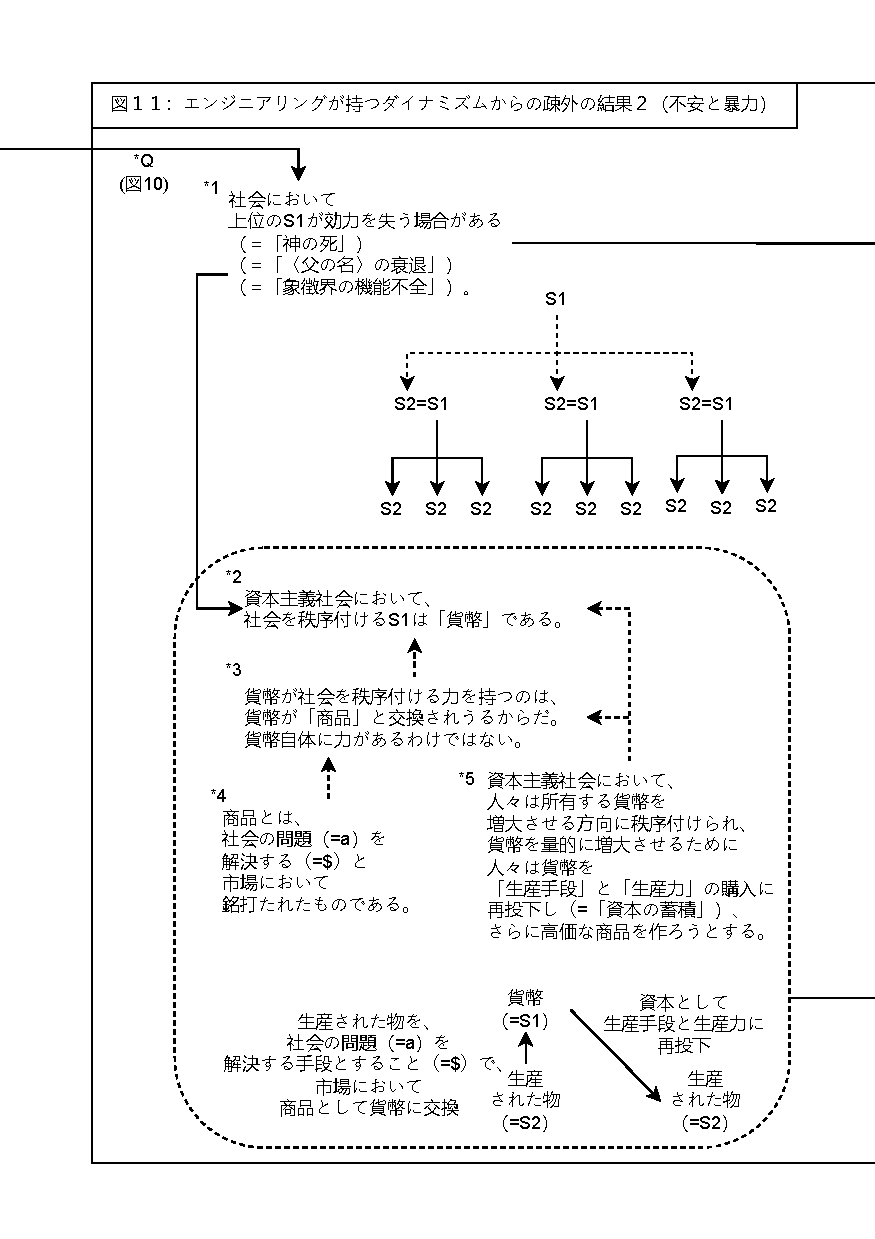
\includepdf[pages=-, scale=0.90, pagecommand={\thispagestyle{plain}}]{../figures/図11.pdf}

\section{結論:人間の限界とその先}

\subsection{結論1:人間の不満と満足が現れるダイナミズムのモデル化}\label{ux7d50ux8ad6uxff11ux4ebaux9593ux306eux4e0dux6e80ux3068ux6e80ux8db3ux304cux73feux308cux308bux30c0ux30a4ux30caux30dfux30baux30e0ux306eux30e2ux30c7ux30ebux5316}

\subsubsection{目標1:四つのあり方と特異性}\label{ux76eeux6a19uxff11ux56dbux3064ux306eux3042ux308aux65b9ux3068ux7279ux7570ux6027}

本稿のここまでの議論から、人間の満足には四つのあり方があることが分かった。ここでは、その四つのあり方を総括していく。四つのあり方のそれぞれでどのように欲動が解消されるかが、それぞれにおける満足のあり方を規定する。そこで特異性の観点を忘れないようにすることが、後の考察を実りあるものにする上で決定的に重要となる。

\subsubsection{根源的な欲動の解消}\label{ux6839ux6e90ux7684ux306aux6b32ux52d5ux306eux89e3ux6d88}

第一のあり方は、\textbf{根源的な欲動}のレベルでの満足である。欲動の解消はあらゆる満足の条件である。その意味では、欲動の満足は第二から第四までのあり方の背後を通底している。欲動の満足は、第二から第四までのあり方は社会的な意味の場で得られるものであるから、非社会的で非意味的な満足だと言うことができる。欲動の満足の具体例としては、「身体を動かすことが(社会的な意味を伴う場合であっても)単にそれ自体で楽しい」とか「声を聞くことが(同じく)単にそれ自体で楽しい」などといったケースが挙げられる。これらは即ち、運動や芸術などによる欲動の解消である。

ここで、\textbf{各人の欲動に備わった特異性}(以下、単に「\textbf{特異性}」と表記)についてて指摘しておくべきことがある。それは、欲動のあり方には人による違いがあり、そして解消困難な欲動を軸に欲望は構築されるということとだ。後に詳しく考察するが、この点を忘れて「新しい物語の『推奨ボーダーライン』」について考察すると、実践的な生き方は導き出せなくなってしまう。

\subsubsection{神経症的な欲望の場の展開}\label{ux795eux7d4cux75c7ux7684ux306aux6b32ux671bux306eux5834ux306eux5c55ux958b}

第二のあり方は、神経症的な欲望の場を展開させることで生じる満足である。これは第三と第四のあり方を可能にする\textbf{基本的な力}を行使する満足である。ここでは「その場を秩序付ける根拠となる項が制定され、その根拠に基づいた秩序が形成された後に、その秩序の不完全さが露呈させられ、また新たな根拠となる項が制定される」といった秩序の構築と放棄の繰り返しが行われる。この繰り返しが持つ意味の変動がもたらす満足が、満足の第二のあり方だ。

この第二のあり方は、秩序が持つ不完全性と密接な関係を保ちながら作用するため、その時々に人が抱える欲動とも近しい関係を維持できる「健康的」なあり方だと言うことができる。その具体例には「それまで解けなかったパズルが解けた(非意味的に現れていた対象を意味の体系へと統合できた)」であるとか「広く正しいと思われていた説明のおかしな点を発見できた(意味の体系が孕む非意味的な対象を露呈させることができた)」などのケースが挙げられる。

ここで、第一のあり方の最後に触れた\textbf{特異性}について、第二のあり方がどのように関わるかの関係を付記しておこう。第二のあり方において、人は秩序の構築と放棄の繰り返しを経験する。すると、この繰り返し通じて、人は自身の欲望が様々に姿を変えることと、そこで欲望が見せる振れ幅の中に「核」になって維持されているような部分がある(「〈一〉部分あり(Y'a
d'l'Un)」)ことに気付くことがある。これが「その人が求めずにはいられないもの」であり、その核の中にその人に特有の欲動があるのだ。こうして「それを知り、それを裏切らないようにする」という境涯が開かれることになる。そして、人はこの境涯において正直になり、自身に嘘を付くことをやめ、罪責感との縁を絶つことができるようになるのだ。

\subsubsection{神経症的な欲望の場における承認}\label{ux795eux7d4cux75c7ux7684ux306aux6b32ux671bux306eux5834ux306bux304aux3051ux308bux627fux8a8d}

第三のあり方は、神経症的な欲望の場が形成するヒエラルキーの中で充足することによる満足である。そこでは超越的な存在(=象徴的父)が措定され(=父性隠喩)、その存在を根拠としてこの世界のあらゆるものが固定された意味を持つようになる(=ファリックな意味作用)。これは世界の全体に効果をもたらす\textbf{権威主義的な世界観}に依拠した満足だと言える。こうした権威主義的な世界観の、最も強力な形態が絶対的な価値秩序を持つ宗教によって提供される世界観であり、世俗的な形態の一つが自明な文化的価値秩序があるとする世界観であり、もう一つが客観的な真理の存在を前提とする(科学的な態度の前提となるような)世界観である。これらはプレモダンな世界観だと言うことができる。そこでは固定された意味それ自体にアクセスできるのは超越的な存在に限られており、人々はその断片を知ることしかできないのだが、それでも「固定された意味が存在する」と信じることは人に安心をもたらす。そして、その安心の中で特定の物事を達成すると、その達成にも意味が与えられることになり、満足も得られる。これは、〈父〉なる存在により「承認」される満足だということもできる。

こうした満足の具体例としては、宗教的な場合では「特定の人物に対する信仰を持つことを公言した。これは死後の救済に必要な行為である。なので私は死後の救いに近づいた。喜ばしい」であるとか「子孫を残すことで先祖は救われる。私は子孫を残すことができたので、先祖に対する孝行を果たした。喜ばしい」などといったケースが挙げられ、また世俗的な場合では「(社会的に『一人前の大人ならば結婚して子供を作るべきだ』と言われている状況下で)それを達成できた。喜ばしい」であるとか「事件の真相が分からず社会が不安であった状況で、真犯人を見つけ出した。これで社会に安心を取り戻すことができた。そこに貢献できて喜ばしい」などといったケースが挙げられる。

この権威主義的な世界観において、構築された秩序は硬直しており、その基礎となる部分に据えられた根拠を放棄するのが難しくなっている。そうした状況の中では、第二のあり方と\textbf{特異性}との関係について論じた際に触れたような「自身の欲望の振れ幅」を知る機会も抑圧されてしまう。こうして第三のあり方は、人を安心させることによって、人を無知の中に置き去りにしてしまう危険性を持つことになる。

\subsubsection{資本主義的な場における不満の排除}\label{ux8cc7ux672cux4e3bux7fa9ux7684ux306aux5834ux306bux304aux3051ux308bux4e0dux6e80ux306eux6392ux9664}

第四のあり方は、権威主義的な世界観において物事の意味や価値を定義していた存在(その最たるものが超越的な存在)が、価値を媒介する項に代替されて不要になることで現れる\textbf{資本主義的な体制}の下で可能となる満足である。このモダンで資本主義的な体制下では、人は自らが持つ価値の媒介を増やすべく、他者に対してその他者持つ欲動を解消する手段を提示し、他者に「その手段が欲しい!」という欲望を抱かせることで、他者が持つ媒介と手段との交換を成立させる。

より資本主義経済の文脈に引きつけた具体例を挙げると、このプロセスは「資本家や労働者は自らが持つ貨幣を増やすべく、他者に対してその他者が持つ不満を解消する商品を提示し、他者に『その商品が欲しい!』という欲望を抱かせることで、他者が持つ貨幣との交換を成立させる」という話においても成立しているといえる(このとき、他者は自身の欲動を欲望にすり替えられることで、消費者へと変化させられている)。こうして人々は、一方では価値の媒介をより多く持とうとすることで他者の不満を発見し解消する運動へと秩序付けられ、他方では自身の不満を解消すべく自身が持つ価値の媒介を他者に差し出し続けることになる。

この資本主義的なプロセスにおいて消費者の位置に置かれた者が晒されている危険は、自身がより深く満足するか否かの熟慮をせずに他者が提示する手段に飛びついてそれを欲望の対象とすることで、欲動を浅いレベルで解消し続けてしまうことにある。もし、そのように振る舞うのであれば、消費者の位置に置かれた者は、第二のあり方のところで述べたような自己理解に至る道を辿ることが困難になってしまう。この意味で、資本主義的なプロセスは人を\textbf{特異性}に向かわせない傾向を持つ。

ただし、資本主義的な体制下での人間の行為には\textbf{特異性}について付け加えておくべき論点がある。それは、資本主義的な体制は、権威主義的な世界観よりも広い範囲の行為を許容しているという点だ。理念的に言えば、権威主義的な世界観の下ではあらゆる行為の意味や価値が固定されており、多くの行動が禁止されている(まさしく、そうした禁止によってプレモダンの秩序は保たれているのだ)。これに対して、理念的には、資本主義的な体制下ではあらゆる行為の意味や価値は貨幣と商品との交換を妨げない限りで許容されている。したがって、自分自身が持ちうる欲望の振れ幅を探究するという行為もまた、資本主義的な体制下では許容されうるのだ。

\newpage

\subsection{結論2:新しい物語の推奨ボーダーライン}\label{ux7d50ux8ad6uxff12ux65b0ux3057ux3044ux7269ux8a9eux306eux63a8ux5968ux30dcux30fcux30c0ux30fcux30e9ux30a4ux30f3}

\subsubsection{目標2-1:論点の整理}\label{ux76eeux6a19uxff12uxff11ux8ad6ux70b9ux306eux6574ux7406}

こうして、満足の四つのあり方を整理することができた。この整理をもとに、ここからは「新しい物語の『推奨ボーダーライン』」について考察していく。そのためには、新しい物語の要件を再確認する必要がある。その要件は、まず第一に物語が解決すべき問題を確認した上で、続いて第二に現代社会における人間と物語との関係を確認することで確認できる。

まず第一に、物語が解決すべき問題について確認する。その問題とは、そこに意味が存在しないことに耐えられないような謎が存在することだ。人が持つ知はシニフィアンの体系に依存しており、そしてシニフィアンの体系は常に不完全なものである以上、人の知も常に不完全であり、それゆえ人は常に謎(対象a)と共にある。そして、謎のうちには、悲惨や苦痛に満ちた、人を途方に暮れさせるものがある。そうした耐えがたい謎を前にして、人は物語を求めるようになるのだ。

続いて第二に、現代社会における人間と物語の関係を確認する。その関係は、冒頭の「問題意識あるいは問いの設定」において「過去より存在する物語を信仰し続けるのには筋金入りの信心が必要であり、ナイーブに未来を信じるのには事態は差し迫りすぎ」ていると記述した通りだ。本稿のここまでの議論とこの記述を踏まえて新しい物語の要件を洗練化させると、それは「科学的知見と整合的であり、人類の未来はナイーブに楽観できるわけではないことを認めた上で、人の生に意味を与える物語」だということになる。そのような新しい物語があれば、それに救われる人もいるだろう。

\subsubsection{目標2-2:考察と方法(1:物語を求める前に)}\label{ux76eeux6a19uxff12uxff12ux8003ux5bdfux3068ux65b9ux6cd5uxff11ux7269ux8a9eux3092ux6c42ux3081ux308bux524dux306b}

それでは、そうした新しい物語は、具体的にどのような科学的知見や未来観に束縛されているのだろうか。その問いに答える前に、\textbf{根源的な欲動}のレベルでの満足に触れておこう。

まず指摘しなければならないのは、「人が常に謎と共に在る」からといって、「人が常に物語を求める」わけではないということだ。実際、意味を求めることなしに欲動が解消され、満足が得られる場合がある。それは第九章で述べたように、運動や芸術などによって人が充実する場合があるからだ。例えば、人は忙しく身体を動かしているとき、意味を求めようとすることを忘れてしまう。また、友人とおしゃべりをしているときや気晴らしにやるゲームに熱中しているときなどには、少なくない人が人生の謎について考えることを忘れている。他にも、芸術作品の制作に熱中したり、あるいは芸術作品をのめり込むように鑑賞している時に、人は自身が抱える謎から距離を取ることができる。そして、いずれの場合でも、人はそれらの行為によって「スッキリ」することができる。この論点から分かることは、人は運動や芸術を通じて欲動を解消することで、向き合うべき謎を軽減し、抱える問題を軽くできるということだ。

身も蓋もない話ではあるが、抱える問題をなるべく軽くすることを軽視してはいけないと筆者は考えている。なぜなら、抱える問題を軽減することを怠れば、その分だけ、その問題を意味を用いて合理化しなければならなくなるからだ。物語を信仰することは、結局のところ合理化であり、現実に対する防衛にすぎない。そして、防衛というのは、情動を消すことができるわけではなく、情動に上書きされる思考を曲げるものにすぎないのだった。だから、合理化すればするだけ、自分自身から目を背けることが増えていく。そうすると、ますます自身を苦境に追い込んでいき、本来ならば抱えずに済んだ問題まで抱えることにもなりかねないわけである。

しかし一方で、運動や芸術によって欲動を解消することについて、哲学は無条件な称揚を避けてきたように見える。この点については、どう考えるべきか。筆者が考えるところによれば、それは、運動や芸術といった手段によってのみ欲動を解消し続けた場合、運動や芸術以外の対象についての知識や思考を発達させることが難しくなるからだ。もしそこで人生についての知識や思考の発達が阻害されれば、いざ自身の生に謎が現れた際になす術がなくなってしまう。

こうした知識や思考の発達が阻害される状況は、運動や芸術への一面的な耽溺のみによって起こるわけではない。実際、\textbf{権威主義的な世界観}の下では「世界の多くの物事に対して固定的な意味が規定され、様々な行動が禁止されていることで、人は知識や思考を発達させる契機を奪われている」のであり、\textbf{資本主義的な体制}の下では「お仕着せの欲望をあてがうことによって欲動を解消させてしまうことで、人は自分自身の欲望の核を探求する必要がなくなり、\textbf{特異性}について知識や思考を発達させる契機を失うよう仕向けられている」のだった。

\subsubsection{「欲動の解消」・「知識と思考の発達」・「特異性の探求」の三面を並立させる方法}\label{ux6b32ux52d5ux306eux89e3ux6d88ux77e5ux8b58ux3068ux601dux8003ux306eux767aux9054ux7279ux7570ux6027ux306eux63a2ux6c42ux306eux4e09ux9762ux3092ux4e26ux7acbux3055ux305bux308bux65b9ux6cd5}

この困難を突破するためには、どうすれば良いのか。言い換えれば、運動や芸術による欲動の解消を活用しつつも、知識や思考を発達させ、その過程で自分自身の\textbf{特異性}を見つけ出していくには、どうすれば良いのか。

そこで注目できるのが、\textbf{資本主義的な体制}の下での\textbf{基本的な力}の行使による秩序の構築と放棄の繰り返しだ。具体的に言えば、労働の場の中で自身の知識や思考を「ああでもない、こうでもない」と試行錯誤を繰り返すということだ。この繰り返しを通じて、人は自身の知識や思考を自然や社会に適応させるために洗練させ続けることができる。特に、\textbf{資本主義的な体制}が労働者に対して発揮する労働への圧力ゆえに、人は自分の限界がどのあたりにあるのかを比較的容易に知ることができる。それは、自分の身体の限界であり、自分の欲望の限界だろう。自分自身に担えるものの重さの上限であり、自分自身が「まだやりたい!」と思える範囲と深さの輪郭だ。それらの限界を知ることで、自分自身の振れ幅を知ることに繋がり、そこから自分自身の「求めずにはいられないもの」が浮かび上がってくる。労働は、自身の核となる部分にある愛を探し求めるプロセスにもなりうるのだ。

とはいえ、もちろんこれは相当に器用な生き方だと言わざるを得ない。何故ならば、そのような生き方を実践するためには、第一に自分が「やりたい」と感じた労働に身を投じるための能力と、第二に自身の限界を速やかに感じ取る能力と、第三に自身の限界を感じ取った際に禍根を残さず速やかに撤収する能力が必要だからだ。それらの能力を身に着けるためにはそれだけで多大な才能と境遇と努力が必要になるだろう。これを万人に可能な生き方だと主張するのには無理がある。

先に述べた隘路を突破するための方法について次点として挙げられるのは、ワーク・ライフ・バランスを保つという月並みなものになるだろう。これは先の方法と比べれば(効率は劣るものの)より人を選ばない方法だと言うことができる。とはいえ、これも万人が選び取れる方法だとは言えないだろう。ワーク・ライフ・バランスを重視するだけの恵まれた労働にありつけない者もいるからだ。これも、この状況をどう改善すれば良いかというテーマだけで長大な考察が必要になってしまう。

そして、この二つの方法を実現できなかった人々だけれでなく、この二つの方法を実現できた人々であっても、人生において途方に暮れてしまう謎に突き当たってしまう場合がある(ヤスパースが述べるところの「限界状況」)。そのような謎に遭遇せずに、あるいはそうした謎に遭遇しても囚われずに上手く生きて死ぬ者は幸福だ。しかし、実際問題として、少なくない人が謎に突き当たって途方に暮れてしまうことになる。そこで初めて、物語が避け難く求められるようになるのだ。

\subsubsection{目標2-2:考察と方法(2:これからの物語)}\label{ux76eeux6a19uxff12uxff12ux8003ux5bdfux3068ux65b9ux6cd5uxff12ux3053ux308cux304bux3089ux306eux7269ux8a9e}

人はそうした限界状況においてどのような物語を求めれば良いのかについて早速考えていきたいところだが、その前に、本稿のそうした問いの立て方に対して当然あって然るべき次の問いに答えておこう。それは、「自分が信じる物語を自分で考えて作るのはナンセンスではないのか」という問いだ。この問いに対して本稿は、「『自分で考えて作り、それを自分で信じる』という行為に矛盾が起こらないような意味内容の物語は存在しうる。そして、そうした物語についてであれば、『自分で考えて作り、それを自分で信じる』を取ることには問題がない」と考えている。確かに、「神の啓示を受ける」ことから創始される啓示宗教などにおいては、「自分で考えて作り、それを自分で信じる」という行為に無理が生じる。しかし、それはあくまでその物語の持つ意味内容がそうした創始に矛盾するからにすぎない。「自分が考えた」という創始の経緯は、「それゆえにその物語は誤っている」という結論を帰結するわけではないのだ。例えば、クトゥルフ神話は創作神話であるが、このことが「クトゥルフ神話は世界の真理を表していない」という命題を証明するわけではない。

それでは改めて、限界状況においてどのような物語を求めれば良いかについて考えていこう。まず本稿が考える\textbf{これからの物語}に対して事実上課せられている制限は、冒頭に述べた通り、「この宇宙の中で起こる出来事について、物語が科学的知見と争わない」というものだ。もちろん、科学的知見と争うこと自由だが、そうした場合には「部外者も認める広い再現性を確認することができない主張」をすることになる。それでも(例えば、「この宇宙の歴史上、ただ一度きりしかその奇跡は起こらないのだ」などといったように)補助理論を追加することで誤りを認めないことは無際限に可能だが、これも冒頭に述べた通りの理由で、本稿はそうした態度を積極的には推奨しない。このように、本稿は「\textbf{これからの物語}は、超越的な領域についてのみ語るべきだ」という推奨ボーダーラインを提案する。

この推奨ボーダーラインに従った場合、物語の側が科学的知見に対して要求できる制限はほとんどないのだが、逆に科学的知見の側が物語に要求する制限はある。即ち、残酷な過去や現在についてだけでなく、科学的知見にしたがって導出される未来予測の範囲についても、\textbf{これからの物語}は遍く「何かしら救いのある」意味を与えられるようになっていなければならないのだ。例えば、現代の科学的知見と宇宙論は、相当高い確度で「この宇宙が永遠に生命の生存を許す場所であり続けることはない」ということを示している。その場合、あらゆる命の系譜は最終的に死と共に終わることになる。まずもって、その絶滅の過程に、\textbf{これからの物語}は意味を与えることができなければならない。他にも、科学的知見が\textbf{これからの物語}に対して要求する制限には様々なものがある(例えば、「他の諸物と同じく、生命現象も物理学の法則に従う」とか、あるいは「自由意志は錯覚である」とか\ldots\ldots)。その個別的な制限についてはここまでの議論を振り返って参照されたい。

こうした科学的知見が課す制限の多さにかかわわらず、\textbf{これからの物語}の具体的な実装は、無数にありうる。ここまで考えた上で、自分の考えと矛盾を来さない(あるいは、矛盾の少ない)既存の宗教を信じることにするのも可能だろう(そこで信じる宗教として啓示宗教を選ぶことも、論理的に可能だ)。あるいは、自分が信じることのできる物語をゼロから作り出すこともできる。

この選択の場面において、万人がその物語を進んで信じたいと思えるのか否かを考慮する必要性は必ずしもない。他の人がどう思うかは、その物語の真偽にも関わらないし、当人がそこに「救い」を見出だせるかにも関わらないからだ。したがって、世界を呪詛するのがその人にとって「救い」に感じられるのなら、そうした物語を選ぶことも可能だ。

\subsubsection{神が存在しないわけではない世界を生きる}\label{ux795eux304cux5b58ux5728ux3057ux306aux3044ux308fux3051ux3067ux306fux306aux3044ux4e16ux754cux3092ux751fux304dux308b}

理性が導けるのはここまでである以上、ここから先は「決めの問題」でしかない。このような結論に落ち着くと、「結局は理性からの(キルケゴールが述べるところの)『跳躍』に縋るしかないのなら、これまで行ってきた科学的知見や\textbf{特異性}についての探究は単なる遠回りだったのではないか?」と思われるかもしれないが、そうではない。

それは第一に、反社会的な嘘をそれと知っていてでっち上げる者は(歴史上これまでずっと)多く存在してきたが、地道な自己理解と科学的知見についての探究はそうした連中が弄する虚偽に騙されるリスクを少しは下げてくれるからだ(その上で、これもまた科学的知見がもたらす知識だが、自信過剰は虚偽に対する耐性を下げるがゆえに慎まねばならないことと、そしてどれほどの鍛錬を積んでも騙されるときは騙されるのだということを肝に銘じておくようにしよう)。

続いて第二に、自身の\textbf{特異性}をよりよく掴んでいれば、無数の物語の中から自身にとってより「しっくり」くる物語を選び取ることも、より容易になるだろうからだ。この意味でも、\textbf{特異性}の探究には効果があるわけだ。

そして第三に、科学的知見と自己理解に至るまでの仕組みについて知ることで、場合によっては物語を避け難く求めるしかない状況に陥りうるのだと理解できるからでもある。つまり、物語を避け難く求めることになるのは必ずしも不勉強や意志薄弱ゆえではないと理解できるからだ。そのように理解することで、どうしようもない状況を「これは本当に、自分にとってはどうしようもない状況なのだ」と自覚しなおすことができ、そこで「決然と」物語を信じるという決定を下せるようになるだろう。

それにしても、人類が生きている論理形式と世界構造が「自由な仕方で、超越的な存在を信じること」を許容するようにできているのは驚嘆すべきことであるように筆者には思われる。それらは何故か「端的にそうなっているから、そうなっているのだ」という仕方でそうなっているのであり、そうである必然性はないからだ。これは「世界が『その背面に神秘が存在する余地がある』という仕方で存在している」ことに対する驚愕である。人間は「神が存在しないわけではない」ような世界に住んでいるのだ。そのような世界に住んでいて、それを考え、求めてしまう時にそれを求めないでいるのは、強情でもあるように筆者には思われる。

\newpage

\section{参考文献}\label{ux53c2ux8003ux6587ux732e}

\subsection{序論}\label{ux5e8fux8ad6}

\begin{itemize}
\tightlist
\item
  フリードリヒ・ニーチェ,三島憲一(訳),1974=1984,『ニーチェ全集 第九巻(第Ⅱ期) 遺された断想(一八八五年秋--八七年秋)』白水社.
\item
  --,木場深定(訳),1887=1940,『道徳の系譜』岩波書店.
\item
  ジャン=フランソワ・リオタール,小林康夫(訳),1979=1989,『ポストモダンの条件』水声社.
\item
  ハンス・ロスリング/オーラ・ロスリング/アンナ・ロスリング・ロンランド,上杉周作/関美和(訳),2018=2019,『FACTFULNESS(ファクトフルネス)
  10の思い込みを乗り越え、データを基に世界を正しく見る習慣』日経BP.
\item
  浅田彰,1983,『構造と力--記号論を超えて』勁草書房.
\item
  市川遊佐,2021,「ラカニアン・アジャイル―『四つのディスクール』から考える中間集団論/組織論としての『スクラム』」(『アレ』Vol.9収録,アレ★Club:240-313).
\item
  落合陽一,2015,『魔法の世紀』PLANETS.
\item
  小泉悠/桒原響子/小宮山功一郎,2023,『偽情報戦争 あなたの頭の中で起こる戦い』ウェッジ.
\item
  津田正太郎,2024,「メディア社会とは何か 1. 国民国家とマスメディア―トイ人」(2024年8月21日取得,\url{https://www.toibito.com/toibito/articles/\%E5\%9B\%BD\%E6\%B0\%91\%E5\%9B\%BD\%E5\%AE\%B6\%E3\%81\%A8\%E3\%83\%9E\%E3\%82\%B9\%E3\%83\%A1\%E3\%83\%87\%E3\%82\%A3\%E3\%82\%A2}).
\item
  松本卓也,2018,『享楽社会論』人文書院.
\end{itemize}

\subsection{第一章}\label{ux7b2cux4e00ux7ae0}

\begin{itemize}
\tightlist
\item
\end{itemize}

\subsection{第二章}\label{ux7b2cux4e8cux7ae0}

\begin{itemize}
\tightlist
\item
  小林武彦,2021,『生物はなぜ死ぬのか』講談社.
\end{itemize}

\subsection{第三章}\label{ux7b2cux4e09ux7ae0}

\begin{itemize}
\tightlist
\item
  乾敏郎・坂口豊,2020,『脳の大統一理論―自由エネルギー原理とはなにか』岩波書店.
\item
  気象庁,2023,「気象庁|過去の気象データ検索」(2024年9月12日取得,\url{https://www.data.jma.go.jp/obd/stats/etrn/view/daily_h1.php?prec_no=44&block_no=00&year=2023&month=08&day=&view=p3}).
\item
  小坂修平,2004,『図解雑学現代思想』ナツメ社.
\end{itemize}

\subsection{第四章}\label{ux7b2cux56dbux7ae0}

\begin{itemize}
\tightlist
\item
\end{itemize}

\subsection{第五章}\label{ux7b2cux4e94ux7ae0}

\begin{itemize}
\tightlist
\item
\end{itemize}

\subsection{第六章}\label{ux7b2cux516dux7ae0}

\begin{itemize}
\tightlist
\item
\end{itemize}

\subsection{第七章}\label{ux7b2cux4e03ux7ae0}

\begin{itemize}
\tightlist
\item
\end{itemize}

\subsection{第八章}\label{ux7b2cux516bux7ae0}

\begin{itemize}
\tightlist
\item
  向井雅明,2016,『ラカン入門』筑摩書房.
\item
  トーマス・クーン,中山茂(訳),1970=1971,『科学革命の構造』みすず書房.
\item
  フレッド・ホイル,中島龍三(訳),1973=1974,『コペルニクス:
  その生涯と業績』法政大学出版局.
\end{itemize}

\subsection{第九章}\label{ux7b2cux4e5dux7ae0}

\begin{itemize}
\tightlist
\item
  市谷聡啓,2018,『カイゼンジャーニー―
  たった1人からはじめて、「越境」するチームをつくるまで』翔泳社.
\item
  今村仁司,2024,『仕事』講談社.
\item
  小田中育生,2023,「Be
  Agile~-アジャイルマインドセットでいきいきと働く-」(2024年10月23日取得,\url{https://speakerdeck.com/ikuodanaka/be-agile-and-work-with-a-iki-iki-spirit})
\item
  斎藤幸平,2023,『マルクス解体―プロメテウスの夢とその先』講談社.
\end{itemize}

\subsection{第十章}\label{ux7b2cux5341ux7ae0}

\begin{itemize}
\tightlist
\item
\end{itemize}

\subsection{第十一章}\label{ux7b2cux5341ux4e00ux7ae0}

\begin{itemize}
\tightlist
\item
\end{itemize}

\subsection{結論1}\label{ux7d50ux8ad6uxff11}

\begin{itemize}
\tightlist
\item
\end{itemize}

\subsection{結論2}\label{ux7d50ux8ad6uxff12}

\begin{itemize}
\tightlist
\item
\end{itemize}

\subsection{結論3}\label{ux7d50ux8ad6uxff13}

\begin{itemize}
\tightlist
\item
\end{itemize}

\newpage

謝辞

\begin{itemize}
\tightlist
\item
  2024-07-27に記載(2024-07-28最終更新):

  \begin{itemize}
  \tightlist
  \item
    この研究は、『アレ
    vol.9』所収の市川遊佐「ラカニアン・アジャイル―『四つのディスクール』から考える中間集団論/組織論としての『スクラム』」を主要先行研究として、サークル〈アレ★Club〉の活動の中で作られた。
  \end{itemize}
\end{itemize}

\newpage

\backmatter
\printindex

\end{document}

